%-------------------------------------------------------------------------------
%
% Eine \LaTeX-Vorlage zum Buch-Style des Springer-Verlages (svmono.cls)
% f�r die deutsche Sprache
%
% Idealerweise zu verwenden mit pdfLatex / Miktex unter Windows
% zusammen mit TexnicCenter
%
% Anm.: Das Template entspricht zu 95 % dem Template f�r Diplomarbeiten gem.
% http://www.formbuch.de , eine ausf�hrliche Anleitung zum Gebrauch findet sich
% im Buch "Form der wissenschaftlichen Ausarbeitung"  (Springer-Verlag)
%
% Autor:            Tilo Gockel
% Versionsnummer:   0.901
% Datum:            12. Mai 2010
%
% Kontakt:          Hochschule Aschaffenburg, Forschungsreferat
%
%                   info@formbuch.de
%                   http://www.formbuch.de
%
%-------------------------------------------------------------------------------

%\documentclass[envcountsame, envcountchap, openany, deutsch, vecarrow]{svmono}
\documentclass[envcountsame, envcountchap, deutsch, vecarrow]{svmonosf}
%-------------------------------------------------------------------------------

% fonts and the like
\usepackage{lmodern}
\usepackage{avant}
\usepackage{fouriernc}

\usepackage{svmonoext}
\usepackage{pgfgantt}
\usepackage{pdflscape}
\usepackage{longtable}

\usepackage{setspace} 
\usepackage{caption}	% Beschriftungen in Breite einschr�nken
\usepackage{wrapfig}
\usepackage{bigdelim}
\usepackage{multirow}
\usepackage{amsmath}
\usepackage[rightcaption]{sidecap}	%Beschriftungen neben Bildern
\usepackage[]{mcode}				% Einbindung von Matlab-Code
%-------------------------------------------------------------------------------
\usetikzlibrary{calc,patterns,decorations.pathmorphing,decorations.markings}

%-------------------------------------------------------------------------------

\def \doctitle {Shock Detection f�r vernetzte Uhren }
\def \docauthor {Bettina Wyss}
\def \docsubject {Subjekt}
\def \docsubtitle {Pipapo}
\def \doclocation {Luzern}
\def \dockeywords {{Stichworte} {Stichworte} {Stichworte}}

\def \doccomment {Hier kann eine Widmung oder ein Spruch eingef�gt werden.}

%-------------------------------------------------------------------------------

\hyperrefsetup{colorlinks=false}

\renewcommand{\baselinestretch}{1.2}

\lstset{%
    basicstyle=\ttfamily,%
    keywordstyle=\color{blue},%
    columns=fixed,basewidth=.5em,%
    commentstyle=\color[RGB]{0,127,0},%
    linewidth=\linewidth,%
    captionpos=b,%
    frame = none,%
    backgroundcolor = \color[RGB]{230,230,230},%
    aboveskip=\intextsep,%
    belowskip = \floatsep,%
    showstringspaces = false,%
    stringstyle = \color[RGB]{163,21,21},%
    tabsize=2,%
    float=[htbp]}

%-------------------------------------------------------------------------------

\makeindex

\bibliographystyle{bibliografie/ka-style}

\begin{document}
\onehalfspacing
%\nocite{*}                     % vollst�ndige bibliographie anzeigen

%-------------------------------------------------------------------------------

\begin{titlepage}

\begin{center}

% Oberer Teil der Titelseite:
%\includegraphics[width=0.15\textwidth]{./logo}\\[1cm]    
\textsc{\LARGE Diplomarbeit}\\[0.5cm]
\textsc{\Large BAA+E.F1601 }\\[2.5cm]

\textsc{\Large Hochschule Luzern\\
    ~\\
    Technik \& Architektur}\\[0.5cm]

\vfill{}

% Title
\newcommand{\HRule}{\rule{\linewidth}{0.5mm}}
\HRule \\[0.4cm]
{   
        ~\\
        \huge \doctitle\\[0.8cm]}
		\large %\docsubtitle\\
%[0.6cm]
\HRule \\[4cm]
\vfill
% Author and supervisor
\begin{minipage}{0.4\textwidth}
    \begin{flushleft} \large
        \emph{Autorin:}\\
        Bettina \textsc{Wyss}\\
    \end{flushleft}
     \vspace{2.2cm}
     \begin{flushleft} \large
     	\emph{Abteilung:} \\
     	Elektrotechnik
     \end{flushleft}
     \vspace{2mm}
     \begin{flushleft} \large
     	\emph{Klassifikation:} \\
     	R�cksprache
     \end{flushleft}
\end{minipage}
\hfill
\begin{minipage}{0.4\textwidth}
    \begin{flushright} \large
        \emph{Industriepartner:} \\
        Moser-Baer AG\\
        Spitalstrasse 7\\
        3454 Sumiswald
    \end{flushright}
    \vspace{1.2cm}
    \begin{flushright} \large
    	\emph{Dozent:} \\
    	 Prof. Zeno  \textsc{St�ssel}
    \end{flushright}
    \vspace{1mm}
    \begin{flushright} \large
    	\emph{Experte:} \\
    	Thomas  \textsc{Schmidiger}
    \end{flushright}
\end{minipage}

\vfill{}
\vfill{}
\vfill{}

% Unterer Teil der Seite
{\large Horw\\ \today}

\end{center}

\end{titlepage}

%\cleardoublepage
\chapter*{Sperrvermerk}
\markboth{Sperrvermerk}{Sperrvermerk}

Die vorliegende Dokumentation enth�lt vertrauliche Informationen der
X AG. Ver�ffentlichungen oder Vervielf�ltigungen -- auch
auszugsweise -- sind daher ohne schriftliche Genehmigung der
X AG nicht gestattet. Die Arbeit ist nur den Korrektoren sowie
den Mitgliedern des Pr�fungsausschusses zug�nglich zu machen.

\medskip
\medskip
\doclocation, den \today

\medskip
der Autor \\
\docauthor

\cleardoublepage
\chapter*{Redlichkeitserkl�rung}
\markboth{Redlichkeitserkl�rung}{Redlichkeitserkl�rung}

Hiermit erkl�re ich, dass ich die vorliegende Arbeit selbstst�ndig angefertigt und keine
anderen als die angegebenen Hilfsmittel verwendet habe. S�mtliche verwendeten Textausschnitte,
Zitate oder Inhalte anderer Verfasser wurden ausdr�cklich als solche gekennzeichnet.

\medskip
\medskip
\doclocation, den \today

\medskip
der Autor \\
\docauthor

\cleardoublepage
\chapter*{Abstract}


	NTP-synchronized clocks have the ability to send a message through the network. It seems useful to
	send an alarm message if a clock has been damaged through vandalism. The aim of this paper is to find out if
	it's possible to detect vandalism with means of acceleration measurement. 
	
	To do that, an
	experimental setup was developed. The central components were three piezoelectric acceleration sensors. The
	experiments with different projectiles provided information about the optimal sensor position, the 
	dimesion an shape of the acceleration signals and if there is a chance to distinguish vandalism from a passing
	train. As a next step a MEMS acceleration sensor has been taken in service as a data logger. This
	showed that the shock detector can be easily and cheaply implemented. Different ideas to integrate the
	shock detector into the existing clock set have been collected. After discussing the pros and cons
	of each idea, the best one has been realized as a shock detector module. 
	
	It's a likely assumption
	that clocks get hit through an object like a stone. Even weak strikes result in large
	accelerations measured by the clockwork. The strike deforms the plastic disk. The air between the
	disk and the clock face is compressed an acts like a spring. Thats the reason why the clock face begins to 
	oscillate at a specific frequency. In comparison to that, the force initiated from a passing by
	train or gust of wind, has an effect on the entire surface of the clock face. The plastic disk doesn't
	deform and the clock face doesn't get stimulated. As a consequence the optimal sensor position is the
	clockwork, which is connected to the clock face. The MEMS acceleration sensor H3LIS331DL with a
	package size of just 3x3x1mm$^3$ is used for realization.
		

%	NTP-synchronisierte Aussenuhren bieten die M�glichkeit, eine Nachricht �ber das Netzwerk
%	abzusetzen. Es ist sinnvoll, dass bei einer durch Vandalismus besch�digten Aussenuhr ein
%	Alarm-Signal �ber das Netzwerk abgegeben werden kann. Es ist abzukl�ren, ob die Erkennung eines
%	solchen Shock Events mittels Beschleunigungsmessung grunds�tzlich m�glich ist.
%	
%	Es wurde ein Messaufbau mit drei piezoelektrischen Beschleunigungssensoren entwickelt, um Shock
%	Events zu simulieren. In Versuchen wurde die optimale Position des Beschleunigungssensors in der
%	Aussenuhr gesucht und abgekl�rt, ob die Detektion eines Shock Events zuverl�ssig realisiert werden
%	kann und beispielsweise von einer Zugdurchfahrt unterscheidbar ist. Zus�tzlich wurde ein MEMS
%	Beschleunigungssensor in Betrieb genommen und ebenfalls am Versuchsaufbau getestet. Verschiedene
%	Ideen, wie ein Shock Detector in den bestehenden Uhrenaufbau integriert werden kann, wurden
%	skizziert und die Vor- und Nachteile diskutiert. Zum Schluss wurde eine Realisierungsidee
%	umgesetzt.
%	
%	Es ist wahrscheinlich, dass bei Vandalismus Aussenuhren mit einem Gegenstand beworfen oder
%	geschlagen werden. Die Versuche haben gezeigt, dass bereits bei schwachen Schl�gen hohe
%	Beschleunigungen an der Aussenuhr zu messen sind. Durch den Schlag wird die sch�tzende
%	Scheibe eingedr�ckt und das dahinter liegende Zifferblatt angeregt, welches nun mit einer
%	bestimmten Frequenz schwingt. Im Gegensatz dazu wirkt die Kraft- ausgel�st durch eine Zugdurchfahrt
%	oder Windb�e- auf der ganzen Scheibenoberfl�che. Die Scheibe wird dadurch kaum deformiert und das
%	Zifferblatt somit nicht angeregt. Die geeignetste Position f�r einen Beschleunigungssensor ist am
%	Uhrwerk. F�r die Realisierung des Shock Detectors wird ein MEMS Beschleunigungssensor
%	eingesetzt. Dieser hat eine Gr�sse von nur gerade 3x3x1mm3.



\cleardoublepage
\tableofcontents

\cleardoublepage \preface

Sensoren werden in unserem Alltag und in der Industrie immer wichtiger. Eine Verbindung zwischen Umwelt und Maschine 
wird so erschaffen. Dies erlaubt der Maschine, auf Ver�nderungen in der Umwelt zu reagieren. Technologien wie die MEMS-Technologie
erm�glichen kleine und g�nstige Sensorl�sungen. Beschleunigungssensoren bieten unz�hlige Anwendungsm�glichkeiten. 
Sie werden in Smartphones, Kameras, Spielzeugen, aber auch in Airbag Systemen oder zum Messen von Vibrationen oder Schocks 
bei Maschinen verwendet. Auch bei NTP-synchronisierten Aussenuhren soll nun die M�glichkeit gepr�ft werden, Vandalismus mittels Beschleunigungsmessung
zu detektieren. Gelingt dies, k�nnen Aussenuhren preisg�nstig mit dem neuartigen Feature "'Schock Detektion"' erweitert werden. 
 

\italictitle{Danksagung}
Ich bedanke mich bei der Moser-Baer AG f�r die angenehme Zusammenarbeit und hierbei besonders bei den 
beiden Herren Michael Sommer und Hansj�rg Rohrer. Sie waren meine Ansprechpartner bei der Moser-Baer AG und
bei meinen Fragen stets sehr hilfsbereit. Weiter m�chte ich mich bei Herrn Prof. Zeno St�ssel f�r die 
fachkompetente Betreuung seitens der Hochschule Luzern Technik \& Architektur bedanken. 
Zu Dank verpflichtet bin ich auch Tobias Pl�ss f�r die Latex-Vorlage und Prof. Leo Suter f�r 
das Lektorat. 

\medskip
\medskip
\doclocation, den \today

\medskip
die Autorin \\
\docauthor




\part{Grundlagen}
\chapter{Anforderungsliste} \label{chap:anforderungen}

Die folgende Liste zeigt die zu Beginn der Arbeit mit dem Industriepartner definierten
Anforderungen. Diese sind in Anforderungen an die Machbarkeitsstudie, und die Anforderungen an das
Produkt unterteilt. Die Anforderungen an das Produkt sind f�r die Machbarkeitsstudie noch nicht
relevant.
\\
\begin{longtable}{p{0.5cm} p{0.5cm} p{8.5cm} p{2cm} } \toprule
	\textbf{Nr.}	&  &\textbf{Anforderung} & \textbf{Priorit�t} \\	
	\midrule
	\endhead
	\multicolumn{3}{l}{\emph{Fortsetzung auf n�chster Seite}}	\\ \bottomrule \endfoot \endlastfoot
	\\
	  &		&\multicolumn{2}{l}{\textbf{Anforderungen an die Machbarkeitsstudie}}							
	\\
	1 & 	&	Es ist zu �berpr�fen, ob mit einem Beschleunigungssensor 
				Vandalismus an einer Uhr (Besch�digung Scheibe, Uhrwerk) 
				erkannt werden kann												& Forderung \\ 
	2 &  	& 	Der Vandalismus muss von Windb�en und der Sog-Druckwelle 
				eines Zuges unterschieden werden k�nnen. 						& Forderung \\		
	3 & 	& 	Es sollen verschiedene Schock-Situationen getestet werden.		& Forderung \\
	  & 3.1	&	Es soll ein geeigneter Messaufbau entwickelt werden, um 
				die Schock-Situationen zu simulieren. 							& Forderung \\
	  & 3.2 & 	Der Messaufbau muss so gew�hlt werden, dass die Messungen 
				reproduzierbar sind. 											& Forderung \\
	4 & 	&	Falls die Detektion m�glich ist, soll ein geeigneter 
				Algorithmus entwickelt werden (z.B. in MATLAB). 				& Forderung \\
	5 & 	& 	Es soll abgekl�rt werden, ob die Implementierung auf dem
				vorhandenem ATMEL- Kontroller realisiert werden kann.			& Forderung \\
	  &	5.1	&	Falls die Implementierung auf dem ATMEL- Kontroller nicht
				realisiert werden kann, muss abgekl�rt werden, welche
				anderen Komponenten ben�tigt werden.							& Forderung \\
	6 &		& 	Der Stromverbrauch der Produkterweiterung soll abgekl�rt und
				dokumentiert werden.											& Forderung \\
	7 & 	& 	Es soll abgekl�rt werden, ob eine vorhandene Schnittstelle 
				(SPI, I2C, UART) verwendet werden kann.							& Forderung \\
	\\
	 &		&\multicolumn{2}{l}{\textbf{Anforderungen an das Produkt}}								
	\\
	1 &		& 	Die Sensorik darf von aussen nicht sichtbar sein.				& Forderung \\
	2 & 	& 	Der Alarm soll mittels SNMP �ber die bestehende Uhrsteuerung
				abgesetzt werden k�nnen.										& Forderung \\
	3 &		&	Die Kosten f�r den Sensor liegen im Breich von 5 bis maximal 10 Fr.
				pro St�ck.														& Forderung \\
	4 & 	& 	Das Sensormodul soll einfach in der Uhr montiert werden k�nnen.
				Die Platzverh�ltnisse sind insofern beschr�nkt, dass die
				Beleuchtung der Uhr nicht gest�rt wird (siehe Anforderung
				Produkt Nr. 1)													& Forderung \\
	5 & 	&	Das Produkt muss bei einer Betriebstemperatur von -30 bis +70�C 
				arbeiten.  														& Forderung \\
	\bottomrule					 	
	\caption{Anforderungen an die Machbarkeitsstudie und an das Produkt} 
	\label{tab:Anforderungen}
\end{longtable}
%-------------------------------------------------------------------------------
% $HeadURL: http://hb9etc.ch/svn/pluess/tex/da_doku/adaptfilt.tex $
% $Revision: 861 $
% $Author: tobias $
% $Date: 2013-12-23 21:15:48 +0100 (Mon, 23 Dec 2013) $
%-------------------------------------------------------------------------------

\chapter{Physikalische Grundlagen} 

Dieses Kapitel beinhaltet eine �bersicht �ber die f�r die Arbeit wichtigen physikalischen Begriffe
Schock, Beschleunigung, Impuls, Kraftstoss und mechanischen Schwingungen sowie �ber die Fourier Analyse
analoger Signale. 

\section{Definition eines Schocks} \index{Schock} 
\begin{wrapfigure}[10]{r}{7cm}
	\centering
	\vspace{-0.8cm}
	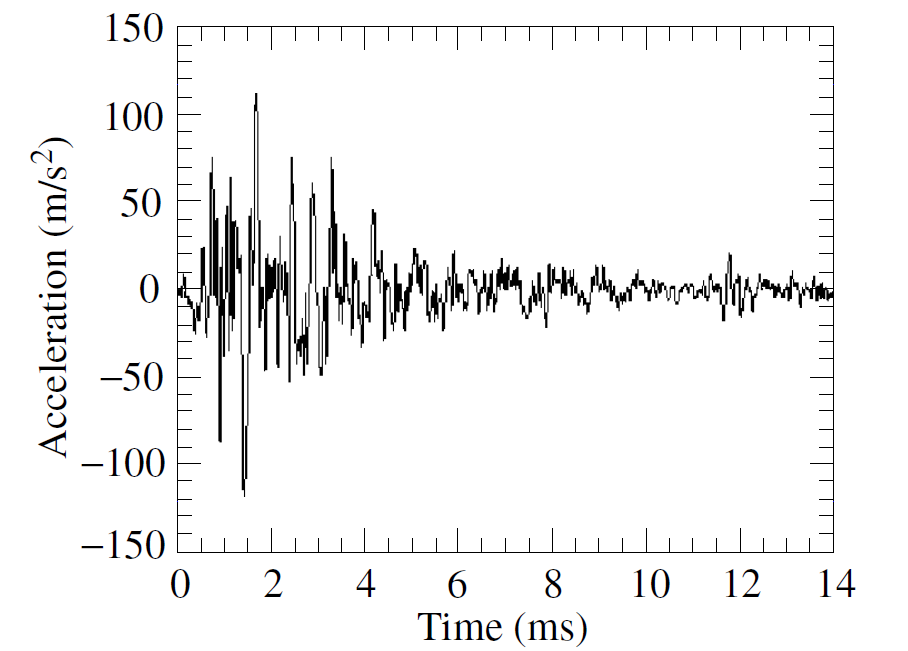
\includegraphics[width=7cm]{img/shock.png}
	\caption[Beispiel eines Schocks]{Beispiel eines Schocks aus \cite{VSH}}
	\label{fig:def_shock}
\end{wrapfigure}
Nach de Silva et al. \cite{VSH} ist ein \textbf{Schock} erfolgt falls sich eine Kraft, eine Position, eine Geschwindigkeit oder eine 
Beschleunigung abrupt �ndert und das betrachtete System in einen transienten Zustand versetzt
wird. Die �nderung wird als abrupt betrachtet, falls diese k�rzer ist als eine nat�rlich 
auftretende �nderung der betrachteten Gr�sse. Die Auswirkung eines Schocks h�ngt einerseits von der Charakteristik 
des Schocks ab (Amplitude, Dauer und Form) und andererseits den dynamischen Eigenschaften des dem Schock 
ausgesetzten Systems. 

\section{Beschleunigung} \label{sec:beschleunigung} \index{Beschleunigung} \index{Mittlere Geschwindigkeit} \index{Momentane Geschwindigkeit}
Der Ort, die Geschwindigkeit und die Beschleunigung eines sich bewegenden Objektes sind 
Vektoren. Sie haben einen Betrag und eine Richtung. Bewegt sich ein Objekt entlang einer Linie x, 
so ist die \textbf{mittlere Geschwindigkeit} das Verh�ltnis zwischen zur�ckgelegtem Weg und Zeit
\begin{equation}
\bar{v}=\frac{\Delta x}{\Delta t}
\end{equation}
wobei $\Delta x$ der zur�ckgelegte Weg und $\Delta t$ die verstrichene Zeit ist. 
Zu einem beliebigen Zeitpunkt ist die \textbf{momentane Geschwindigkeit}  die Weg-Zuwachs-Rate und definiert zu:
\begin{equation}
\vec{v}=\frac{d\vec{x}}{dt}.
\end{equation}

Bewegt sich ein Objekt nicht gleichm�ssig, sondern seine Geschwindigkeit �ndert sich, so erf�hrt
das Objekt eine \textbf{Beschleunigung}. Die Beschleunigung ist somit ein Mass der Geschwindigkeit der 
Geschwindigkeit, die Geschwindigkeits-Zuwachs-Rate
\begin{equation}
\vec{a}=\frac{d\vec{v}}{dt}=\frac{d^2\vec{x}}{dt}.
\end{equation}
Die �nderung der Geschwindigkeit ben�tigt nach Newtons zweitem Axiom die Einwirkung einer 
Kraft (vgl. \autoref{sec:impuls}).

Der Zusammenhang der Gr�ssen durch Differentiation gilt auch umgekehrt. So kann die Geschwindigkeit
oder die zur�ckgelegte Strecke durch Integration der Beschleunigung bzw. Geschwindigkeit berechnet
werden.
	
Bewegt sich ein Objekt auf einer Bahnkurve, wird die Rotation durch die \textbf{Winkelgeschwindigkeit} \index{Winkelgeschwindigkeit}
beschrieben. Sie ist das Verh�ltnis zwischen zur�ckgelegtem Winkel und verstrichener Zeit
\begin{equation}
\omega=\frac{d\Theta}{dt}.
\end{equation}
In jedem Moment besitzt das rotierende Objekt eine lineare Geschwindigkeit v, welche die Richtung
tangential zur Bahnkurve hat. Sie h�ngt davon ab, wie weit das rotierende Objekt vom Zentrum der 
Bahnkurve entfernt ist.  
\begin{equation}
\vec{v}=\omega r
\end{equation}
Bei einem rotierenden Objekt mit konstanter Winkelgeschwindigkeit ist der Betrag der Geschwindigkeit v konstant, die 
Richtung �ndert sich jedoch kontinuierlich. Deshalb erf�hrt das Objekt eine Beschleunigung, welche in die Richtung 
des Zentrums der Bahnkurve zeigt, die \textbf{Zentripetalbeschleunigung.} \index{Zentripetalbeschleunigung} \index{Erdbeschleunigung}
\begin{equation}
a_{ZP}=\frac{v^2}{r}= \omega^2\cdot r 
\end{equation} 

Die \textbf{Erdbeschleunigung} g setzt sich aus zwei Komponenten zusammen: die Anziehung der
Massen und der Rotationsbeschleunigung aufgrund der Erdrotation. In dieser Arbeit 
wird f�r g jeweils der mittlere Wert von 9.81$\frac{m}{s^2}$ angenommen.  
(Aus \cite{ModernSensor})
\section{Impuls und Kraftstoss} \label{sec:impuls} \index{Bewegungsgleichung} \index{Impuls} 
Die Beschreibung, wie sich K�rper bewegen, wird mit den drei Axiomen von Newton 
erweitert. Dabei wird die Frage beantwortet, warum sich etwas bewegt. Ein 
K�rper �ndert seine Geschwindigkeit (Beschleunigung) unter Einwirkung einer
Kraft. Dies widerspiegelt sich in der \textbf{Bewegungsgleichung} (zweites Axiom)
\begin{equation}
\vec{F}=m\cdot \vec{a}.
\end{equation}
Eine weitere Beschreibung der Bewegung eines K�rpers ist der \textbf{Impuls}. Er ist das 
Produkt von Masse und Geschwindigkeit. 
\begin{equation}
\vec{p}=m\cdot\vec{v} 
\end{equation}
Das erweiterte Newtonsche Gesetz lautet somit
\begin{equation}
\vec{F}=m\cdot \vec{a} = m\frac{d\vec{v}}{dt}=\frac{d\vec{p}}{dt}
\end{equation}
und l�sst nun auch ver�nderbare Massen zu. Der \textbf{Kraftstoss} $\vec{J}$ ist \index{Kraftstoss}
die Fl�che unter der Kraft-Zeit-Kurve. Er entspricht der Impuls�bertragung. 
\begin{equation}
\vec{J} = \int_{t_1}^{t_2} \! \vec{F}(t) \, \mathrm{d}t = \vec{p}_2 - \vec{p}_1
\end{equation}
Aus dem Kraftstoss l�sst sich eine durchschnittlich wirkende Kraft berechnen (\autoref{fig:druchschnittskraft})
	\begin{figure}
		\centering
		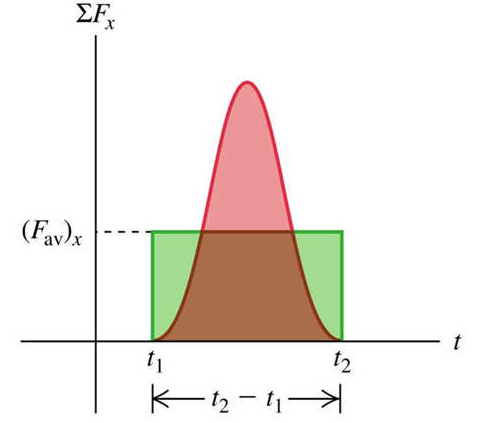
\includegraphics[width=4.5cm]{img/durchschnittskraft.png}
		\caption[Durchschnittliche Kraft $F_{av}$]{Durchschnittliche Kraft $F_{av}$ \cite{Mechanik}}
		\label{fig:druchschnittskraft}
	\end{figure}
	\vspace{-1cm}
\begin{equation}
\vec{F}_{average} = \frac{\vec{J}}{\Delta t} = \frac{\vec{p}_2 - \vec{p}_1}{t_2- t_1} . 
\end{equation}
Ein Impuls�bertrag kann bei kurzen, heftigen St�ssen oder langen, sanften St�ssen 
gleich gross sein. Die Form des Impulses h�ngt von der Steifigkeit der Materialien ab, welche aufeinander treffen. 
%\begin{wrapfigure}[0]{r}{4.55cm}
%	\vspace{1.2cm}
%	\centering
%	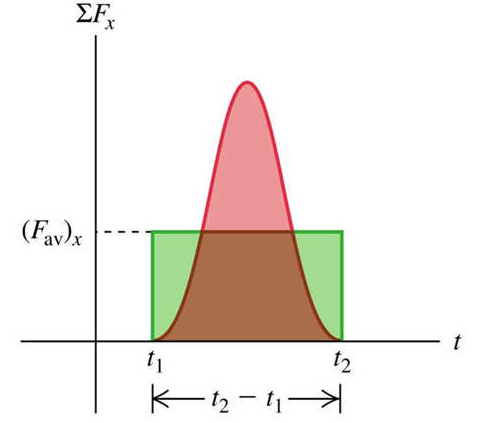
\includegraphics[width=4.55cm]{img/durchschnittskraft.png}
%	\caption[Durchschnittliche Kraft $F_{av}$]{Durchschnittliche Kraft $F_{av}$ \cite{Mechanik}}
%	\label{fig:druchschnittskraft}
%\end{wrapfigure}
Ein steiferes Material erzeugt einen schmaleren Impuls. Die durchschnittliche 
Kraft $F_av$ wird dadurch gr�sser. Das Energiedichtespektrum wird umso breiter, je schmaler der 
Impuls ist. Diese Zusammenh�nge zeigt die \autoref{fig:kraftstoss}. (Abschnitt basierend auf dem Unterrichtsskript Physik der Hochschule Luzern \cite{Mechanik} und \cite{Ruhm})
	\begin{SCfigure}
		%\vspace{0.2cm}
		\centering
		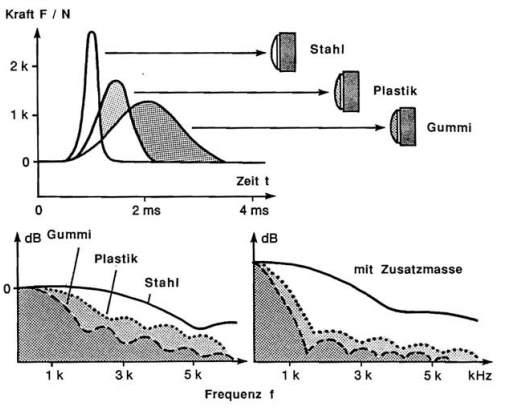
\includegraphics[width=10cm]{img/kraftstoss.png}
		\caption[Kraftstoss]{Die Form des Impulses h�ngt von der Steifigkeit des Materials ab. 
			Je steifer ein Material, desto schmaler der Impuls. Daraus folgt, dass das Energiedichtespektrum
			breiter wird \cite{Ruhm}.}
		\label{fig:kraftstoss}
	\end{SCfigure}
	
	
\newpage
\section{Schwingungen} \index{Periodische Bewegung} \index{Schwingung} \index{R�cktreibende Kraft} \index{Elongation} \index{Amplitude} \index{Harmonische Schwingung}
	Ein K�rper bewegt sich \textbf{periodisch}, wenn er nach gleichlangen Zeitabschnitten immer wieder den 
	gleichen Bewegungszustand einnimmt. Dies heisst, der K�rper erreicht periodisch den gleichen Ort
	mit der gleichen Geschwindigkeit und Beschleunigung. Die Bewegung des K�rpers heisst Schwingung, 
	wenn zus�tzlich eine stabile Gleichgewichtslage vorhanden ist. Ohne �ussere Einfl�sse kehrt 
	der K�rper immer wieder in die Gleichgewichtslage zur�ck. Eine \textbf{Schwingung} kommt zustande, wenn eine 
	\textbf{r�cktreibende Kraft} den K�rper in Richtung der Gleichgewichtslage bewegt. Ist diese r�cktreibende 
	Kraft proportional zur Elongation, so entsteht eine \textbf{harmonische Schwingung}
	\begin{equation}
	x(t) = \hat{x} \cdot cos(\omega t \pm \phi).
	\end{equation}
	Die Periodendauer $T$ ist die Dauer, bis 
	der K�rper wieder den gleichen Bewegungszustand einnimmt. Die Frequenz ist der Kehrwert der Periodendauer
	$f=\frac{1}{T}$ mit der Einheit Herz Hz. Die Kreisfrequenz $\omega$ ergibt sich aus 
	\begin{equation}
	\omega = 2\cdot \pi \cdot f. 
	\end{equation}
	Die \textbf{Elongation} $x(t)$ ist der von der Ruhelage aus gemessene
	Abstand. Die Amplitude $\hat{x}$ ist der maximal Wert der Elongation und ist immer positiv. (Aus
	\cite{MSLeifi} und \cite{Schwingungen})
	
\section{Grundmodell des Masse-D�mpfer-Feder-Prozesses} \index{Masse-D�mpfer-Feder-Prozess}
	Das Grundmodell des Masse-D�mpfer-Feder-Prozesses ist ein lineares System zweiter Ordnung. Es ist
	die Grundlage aller schwingungsf�higen Prozesse h�herer Ordnung. Es ist in
	\ref{fig:feder_masse_daempfer} dargestellt. Die Eingangsgr�sse ist eine angreifende Kraft $f(t)$,
	welche ber�hrungslos auf das System einwirkt.
	\begin{figure}
		\centering
		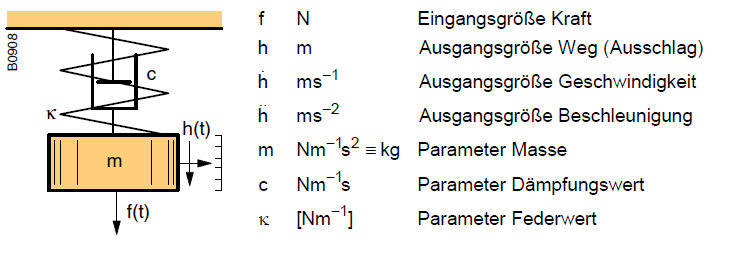
\includegraphics[width=10cm]{img/feder_masse_daempfer.png}
		\caption[Einfachster Masse-D�mpfer-Feder Prozess]{Einfachster Masse-D�mpfer-Feder Prozess \cite{Ruhm}}
		\label{fig:feder_masse_daempfer}
	\end{figure} 
	\begin{figure}
		\centering
		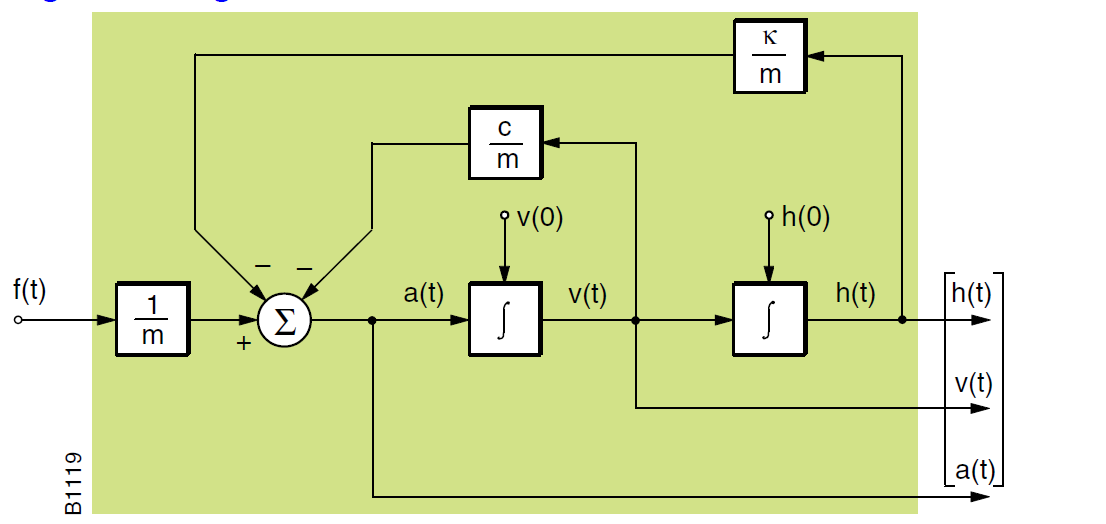
\includegraphics[width=10cm]{img/wirkungsplan.png}
		\caption[Wirkungsplan]{Wirkungsplan, in Anlehnung an \cite{Ruhm}}
		\label{fig:wirkungsplan}
	\end{figure} 
	Das Modell besteht aus physikalischen Gr�ssen ($a$,$v$,$h$,$f$) und physikalischen Eigenschaften
	als Parameter ($c$, $\kappa$, $m$). Um das Modell herzuleiten, wird eine Kr�ftebilanz bei
	oszillierenden Massen durchgef�hrt. Diese besagt, dass zu jedem Zeitpunkt die angreifenden Kr�fte
	im Gleichgewicht sein m�ssen. Dies sind die Massenkr�fte $f_M(t)$ nach Newton, die zur
	Geschwindigkeit proportionalen D�mpfungskr�fte $f_D(t)$, die r�cktreibenden Federkr�fte $f_F(t)$
	und die externen Kr�fte $f(t)$.
	\begin{equation}
	f_M(t) + f_D(t) + f_F(t) = f_F(t) = m\ddot{h}(t)+c\dot{h}(t)+\kappa h(t) = ma(t)+cv(t)+\kappa h(t) = f(t)
	\end{equation}
	\begin{equation}
	a(t) + \frac{c}{m}v(t)+\frac{\kappa}{m}h(t) = \frac{1}{m}f(t)
	\end{equation}
	Der Wirkungsplan ist in \ref{fig:wirkungsplan} abgebildet. Die Struktur bei Mehrmassensystemen, Systemen 
	h�herer Ordnung, �ndert sich nicht. Die urspr�ngliche Bewegungsgleichung wird als Matrix-Vektor-Gleichung
	dargestellt: 
	\begin{equation}
	 \boldsymbol{M\ddot{h}(t)+C\dot{h}(t)+K h(t) = f(t)}. 
	\end{equation}
	(In Anlehnung an \cite{Ruhm})
	
\section{Fourier Analyse analoger Signale} \index{Satz von Fourier} \index{Spektrum} \index{Grundfrequenz} \index{Spektrum!kontinuierliches} \index{Spektrum!diskretes}
	Der Satz von Fourier besagt, dass sich jede periodische Schwingung aus mehreren harmonischen Schwingungen 
	zusammensetzen l�sst. Die Periode der Schwingung heisst \textbf{Grundfrequenz $f_0$}. Alle weiteren enthaltenen 
	harmonischen Schwingungen haben eine Frequenz $f_n> f_0$ und sind ein Vielfaches von $f_0$. Das Betragsspektrum 
	zeigt, welche Frequenzen mit welcher Amplitude in der Schwingung enthalten sind. Das Spektrum einer periodischen 
	Schwingung ist ein \textbf{diskretes Linienspektrum}. Das diskrete Linienspektrum der periodischen Rechteckfunktion ist
	im rechten Teilbild von \autoref{fig:dis_spec_rect}.
	\begin{figure}
		\centering
		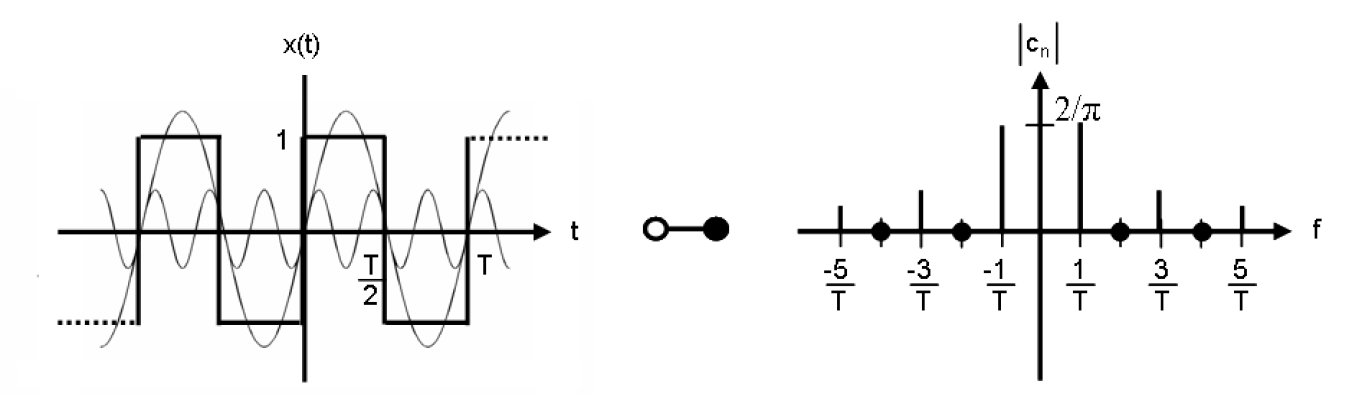
\includegraphics[width=12cm]{img/spektrum.png}
		\caption[Diskretes Linienspektrum einer periodischen Schwingung]{Diskretes Linienspektrum einer periodischen Schwingung \cite{Wassner}}
		\label{fig:dis_spec_rect}
	\end{figure} 
	Aus der Erweiterung der obigen �berlegungen auf aperiodische Signale folgt, dass das Spektrum 
	aperiodischer Signale kontinuierlich ist. Aperiodisch bedeutet, dass die Periode $T$ gegen 
	unendlich strebt, somit $f_0$ gegen null strebt. Die diskreten Frequenzen r�cken deshalb unendlich
	dicht aneinander. (In Anlehnung an \cite{Wassner})

\section{Druck-Sogwellen eines Zuges} \label{Durck-Sogfeld} \index{Sog-Druck Feld}
	Ein vorbeifahrender Zug erzeugt ein Druck-Sogfeld. Dieses ist in der \autoref{fig:SogDruckFeld}
	dargestellt. Die roten Wellen bezeichnen den �berdruck, die blauen Wellen den Unterdruck. Das
	Sog-Druck Feld ist mit dem Zug verbunden und bewegt sich mit der gleichen Geschwindigkeit voran.
	Das Druckfeld nimmt mit der Zuggeschwindigkeit im Quadrat zu. Es ist umso kleiner, je gr�sser der
	Abstand vom Messpunkt zum Zug ist \cite{Niemann}.
	
	\begin{figure}
		\centering
		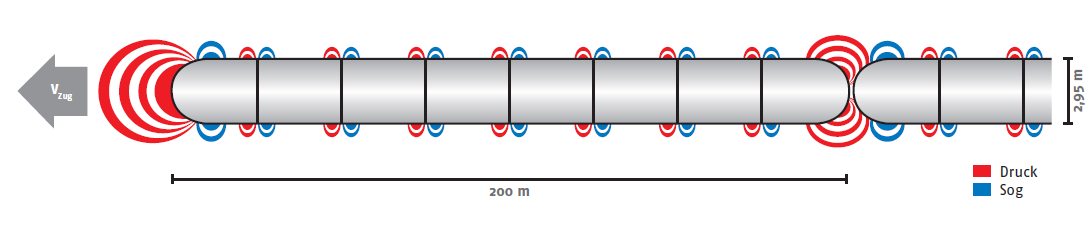
\includegraphics[width=15cm]{img/ZugDruckwelle.png}
		\caption[Typische Druck-Sog-Welle um einen Zug]{Typische Druck-Sog-Welle um einen Zug mit Geschwindigkeit $v_{Zug}$ aus \cite{Niemann}}
		\label{fig:SogDruckFeld}
	\end{figure}	
	Ein typischer Druckverlauf bei einem vorbeifahrenden Zug ist in der \autoref{fig:verlaufDruckwelle}
	gezeigt. Bei der Anfahrt des Zuges wird ein Druck-Sogwechsel gemessen, bei der Ausfahrt des Zuges
	einen Sog-Druckwechsel. In diesen Momenten entstehen die gr�ssten Druckdifferenzen. Ebenfalls grosse
	Druckdifferenzen k�nnen bei den Kupplungsstellen der Zugzeile gemessen werden \cite{Niemann}.
	\begin{SCfigure}
		\centering
		\vspace{-0.5cm}
		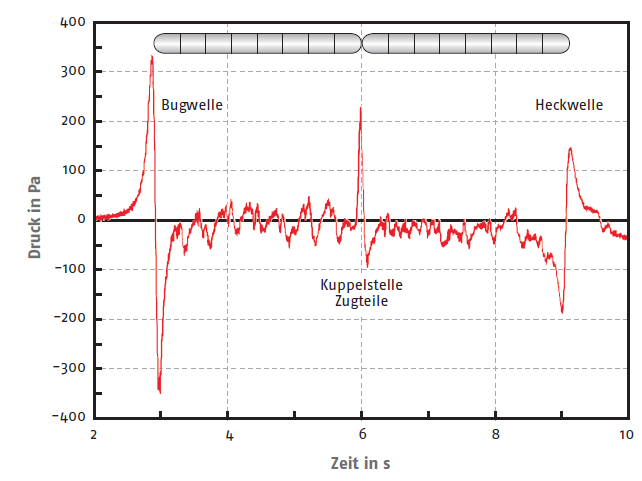
\includegraphics[width=8cm]{img/VerlaufDruckwelleZug.png}
		\caption[Typische Druck-Sog-Welle um einen Zug]{Typischer Druckverlauf bei einem vorbeifahrenden Zug aus \cite{Niemann}}
		\label{fig:verlaufDruckwelle}
	\end{SCfigure}
	Der Abstand zwischen Durck- und Sogwelle L h�ngt nicht von der Zugsgeschwindigkeit $v_{Zug}$ ab,
	jedoch vom Wandabstand zur Gleisachse $a_g$. 
	Der empirische Zusammenhang zwischen Wandabstand $a_g$ und Abstand L wurde von Niemann et. Al \cite{Niemann} hergeleitet: 
	\begin{equation}
	L=6.9 \cdot (\frac{a_g}{3.8})^{0.65} \label{calc:DruckSogAbstand}
	\end{equation}
	Die \autoref{fig:drucksog} zeigt den Zusammenhang graphisch. 
	\begin{SCfigure}
		\centering
		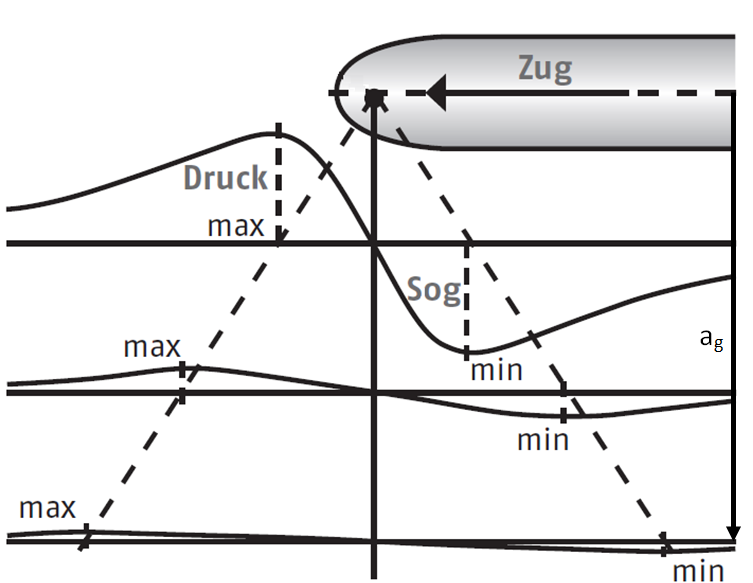
\includegraphics[width=6cm]{img/drucksog.png}
		\caption[Empirischer Zusammenhang zwischen Wandabstand und Druck-Sog-Abstand]{Empirischer Zusammenhang zwischen Wandabstand und Druck-Sog-Abstand aus \cite{Niemann}.}
		\label{fig:drucksog}
	\end{SCfigure}
	Bei zugnahen W�nden wird von $L=6.9m$ ausgegangen. 
	Im Gegensatz zum Abstand L ist der zeitliche Abstand von $v_{Zug}$ abh�ngig. Bei der maximalen Durchfahrtsgeschwindigkeit an Bahnh�fen von 200km/h
	betr�gt diese somit im Minimum $\Delta t = \frac{s}{v}=124ms$. Je gr�sser der Wandabstand, desto gr�sser der Abstand 
	zwischen Durck- und Sogwelle und desto l�nger wird auch der zeitliche Abstand. Somit wird die dynamische Anregung verl�ngert \cite{Niemann}. 
	F�r Systeme mit einer Eigenfrequenz oberhalb der dynamischen Anregung sinkt dadurch die Gefahr zu schwingen. 
\include{l�sungsans�tze}
\include{beschleunigungsmessung}
\include{messmethoden}

\part{Kl�rung der Machbarkeit}
\chapter{Versuche mit piezoelektrischen Sensoren} \label{chap:piezo}
	In einem ersten Schritt wurden Versuche mit piezoelektrischen Sensoren durchgef�hrt. Der
	Versuchsaufbau wird in \autoref{chap:Versuchsaufbau} beschrieben. Es folgen drei Versuche in den
	Abschnitten \ref{subsec:signale} bis \ref{sec:Unterscheidung}: Der erste hat das Ziel, eine
	Vorstellung von den zu messenden Beschleunigungssignalen bei Vandalismus zu geben. Der zweite
	Versuch untersucht die beste Positionierung eines Beschleunigungssensors in der Aussenuhr. Der
	dritte Versuch soll zeigen, ob die Unterscheidung zwischen einer Sog-Druckwelle eines Zuges und
	Vandalismus anhand von Beschleunigungssignalen m�glich ist. Die Versuche sind jeweils in drei
	Abschnitte Vorgehen, Messresultate und Fazit eingeteilt.

	\section{Versuchsaufbau mit piezoelektrsichen Sensoren} \label{chap:Versuchsaufbau}
	\begin{wrapfigure}[10]{r}{6.5cm}
		\centering
		\vspace{-1cm}
		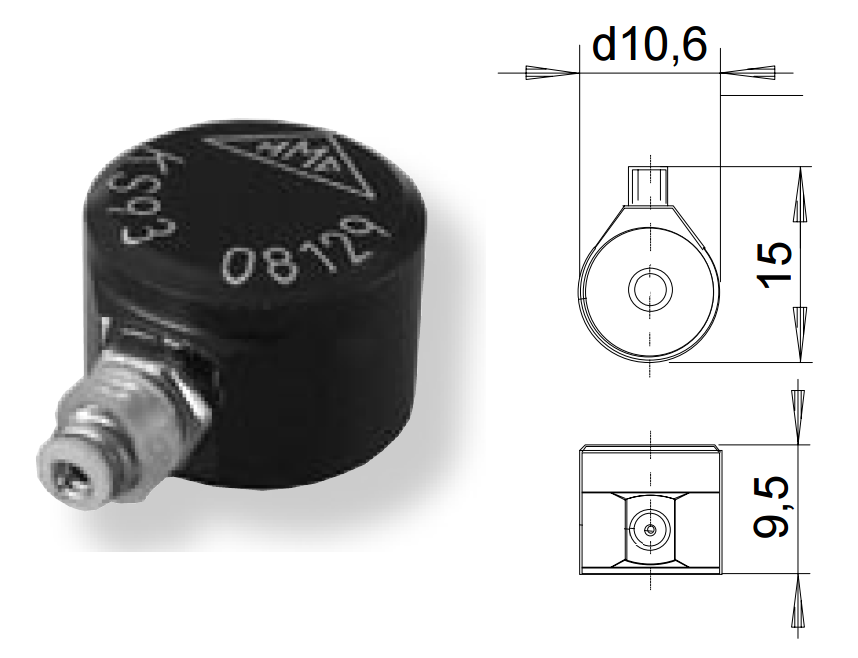
\includegraphics[width=5.5cm]{img/ks93.png}
		\caption{Miniatursensor KS93}
		\label{fig:ks93}
	\end{wrapfigure}
   
	F�r die ersten Versuche werden piezoelektrische Sensoren des Typs KS93 verwendet. Dieser
	\index{Beschleunigungssensor!piezoelektrisch} Miniatur-Beschleunigungsaufnehmer hat einen
	Messbereich von $\pm 6000$g und einen linearen Frequenzbereich bis 22kHz. Der Sensor h�lt
	Beschleunigungen bis maximal 8'000g aus. Am Sensorausgang �ndert sich je nach Beschleunigung die
	Ladung Q. Diese muss mit einem Ladungsverst�rker in eine Spannung umgewandelt und verst�rkt werden.
	Der Ladungs�bertragungsfaktor betr�gt 4.875 pC/g. Weiter Eigenschaften des Sensors KS93 sind dem
	Datenblatt zu entnehmen \cite{KS93}. Der Aufbau und die Funktionsweise von piezoelektrischen 
	Beschleunigungssensoren findet man im Grundlagenteil Beschleunigungssensoren \autoref{chap:acc_sens}. 

	Der Aufbau mit Versuchsuhr, Ladeverst�rker und Oszilloskop ist in der
	\autoref{fig:versuchsaufbau_piezo} dargestellt. Die Versuchsuhr ist liegend an der Wand befestigt,
	so dass die Pr�fmassen auf die Uhr fallen gelassen werden k�nnen. Im Innenraum der Uhr werden drei
	Sensoren befestigt. Die Positionen dieser sind in der \autoref{fig:Sensorpositionen} ersichtlich.  
	Die Sensorpositionen sind so ausgew�hlt, dass der Sensor von aussen nicht sichtbar ist. Dies 
	ist gem�ss der Anforderungsliste in \autoref{chap:anforderungen} erforderlich. 
	Das Signal wird mit dem Ladungsverst�rker M68D3 gewandelt. F�r die Aufzeichnung des Signalverlaufs 
	wird ein Oszilloskop verwendet.	Die aufgenommenen Beschleunigungssignale werden als Bilddatei und als Daten
	f�r Matlab exportiert. Auf dem Computer k�nnen die Messungen ausgewertet werden.
	
	\begin{figure}
		\centering
		%\vspace{-1cm}
		%\captionsetup{width=10cm}
		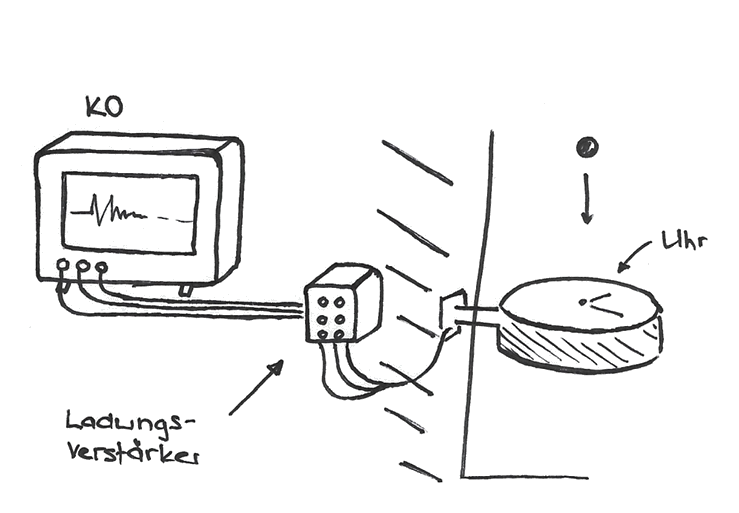
\includegraphics[width=10cm]{img/versuchsaufbau_piezo.png}
		\caption{Versuchsaufbau mit piezoelektrischen Sensoren}
		\label{fig:versuchsaufbau_piezo}
	\end{figure}
	
	\begin{figure}
		%\vspace{1cm}
		\centering
		\captionsetup{width=8cm}
		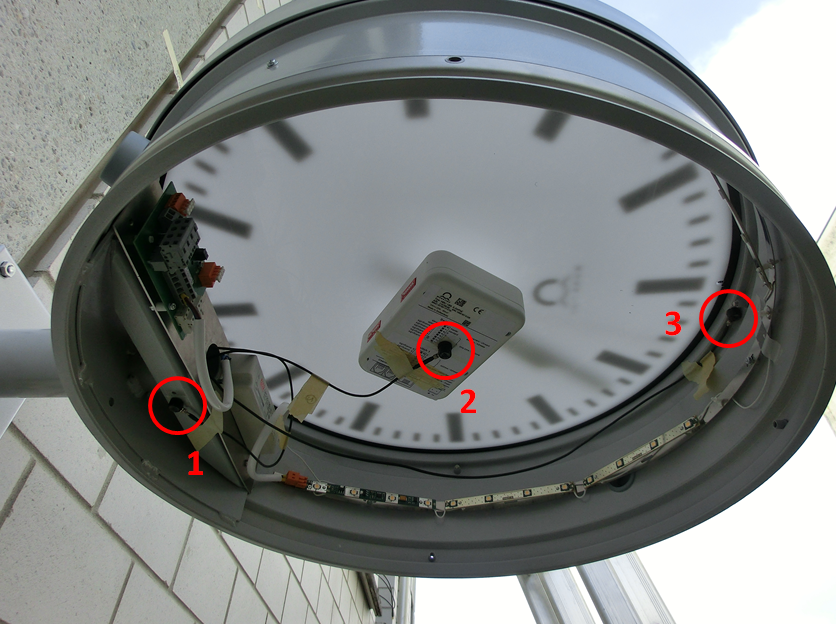
\includegraphics[width=8cm]{img/PosSensoren.png}
		\caption[Sensorpositionen]{Sensorpositionen:\\\\
			1) An der Montageleiste der Uhr innen, nahe der Konsole (Channel 1, gr�n)\\\\
			2) Am Uhrwerk, welches am Ziffernblatt befestigt ist (Channel 2, rot)\\\\
			3) Am Rahmen der Uhr aussen (Channel 3, blau)}
		\label{fig:Sensorpositionen}
	\end{figure}
	
%	\begin{longtable}{p{3cm} p{6cm} p{1.5cm}} \toprule
%		\textbf{Ger�t}	& \textbf{Bezeichnung} & \textbf{Anzahl} \\	
%		\midrule
%		\endhead
%		\multicolumn{2}{l}{\emph{Fortsetzung auf n�chster Seite}}	\\ \bottomrule \endfoot \endlastfoot 
%		Piezoelektrsiche Sensoren	&Miniatur-Beschleunigungsaufnehmer 	KS93&	3	\\ 
%		Ladungsverst�rker			&Messverst�rker M68D3 3 Kan�le			&	1	\\
%		Oszilloskop					&LeCroy									&	1	\\
%		\bottomrule					 	
%		\caption{Verwendete Sensoren und Ger�te} 
%		\label{tab:SensorenGer�te}
%	\end{longtable}
	
	Die vom Oszilloskop exportierten Daten werden in Matlab importiert. Damit nicht bei jeder
	Auswertung die Daten manuell importiert werden m�ssen, wurde eine Funktion readOszData()
	implementiert. Der Code der Matlabfunktion ist im Folgenden abgebildet. Mit der Funktion wird die
	gew�nschte Textdatei ge�ffnet (Zeile 12-15) und Daten in einer Datenstruktur gespeichert (Zeile
	18-22).
	\newpage
	\lstset{
		basicstyle=\small\ttfamily,
		language=Matlab,                % choose the language of the code
		numbers=left,                   % where to put the line-numbers
		stepnumber=1,                   % the step between two line-numbers.        
		numbersep=5pt,                  % how far the line-numbers are from the code
		backgroundcolor=\color{white},  % choose the background color. You must add \usepackage{color}
		showspaces=false,               % show spaces adding particular underscores
		showstringspaces=false,         % underline spaces within strings
		showtabs=false,                 % show tabs within strings adding particular underscores
		tabsize=2,                      % sets default tabsize to 2 spaces
		captionpos=b,                   % sets the caption-position to bottom
		breaklines=true,                % sets automatic line breaking
		breakatwhitespace=true,         % sets if automatic breaks should only happen at whitespace
		frameround=tttt,				% sets round corners
		frame=single,					% with frame
		title=\lstname,                 % show the filename of files included with \lstinputlisting;
	}
	\lstinputlisting[]{code/readOszData.m}
	Der am Oszilloskop aufgenommen Verlauf ist ein Spannungsverlauf welcher dem Beschleunigungsverlauf entspricht. 
	Die Spannung ist Abh�ngig vom Ladungs�bertragungsfaktor und der eingestellten Verst�rkung am Ladungsverst�rker ab. 
	Die Umrechnung von der Spannung in die Beschleunigung in g wird mit der Matlabfunktion 
	volt2acc() automatisiert. Dabei kann die eingestellte Verst�rkung am Ladungsverst�rker als Parameter mitgegeben werden. 
	\lstinputlisting{code/volt2acc.m}
	In Matlab werden die Daten dargestellt und beschriftet. Das Frequenzspektrum wird mit Hilfe des 
	Matlab Tools SPTool erzeugt und analysiert. 
\newpage		
	\section{Zu erwartende Signale bei Vandalismus} \label{subsec:signale}
		\paragraph{Vorgehensweise}
		Unter Vandalismus wird die mutwillige Zerst�rung verstanden, bei der es um eine Zerst�rungslust
		ohne weiteren Zweck geht. So lautet die Definition von Vandalismus auch \flqq absichtliche
		grundlose Zerst�rung \frqq. Nach dem Sprayen (62.5\%, absolut 4726 F�lle im Jahr 2015 im Kanton
		Bern) ist das Ein- und Zerschlagen (8\%, absolut 605 F�lle im Jahr 2016 im Kanton Bern) die
		h�ufigste bekannte Vorgehensweise bei Vandalismus \cite{KSB}. Es wird davon ausgegangen, dass in
		den meisten F�llen die Aussenuhr mit Steinen oder �hnlichen Gegenst�nden beworfen oder geschlagen wird. 
		Deshalb wird der folgende Versuch mit zwei verschieden schweren 
		Stahlkugeln durchgef�hrt. Die beiden Kugeln haben eine Masse von 256g und 537g und entsprechen 
		somit einem kleineren und gr�sseren Stein. 

		\paragraph{Messresultate}
		Die gr�ssten gemessenen Beschleunigungssignale ohne Scheibenbruch sind in \autoref{fig:max}
		dargestellt. Der Beschleunigungssensor am Uhrwerk misst einen maximalen Beschleunigungspeak von -660g! 
		Betrachtet man die Signale im Frequenzbereich, stechen zwei Frequenzen bei ungef�hr 13Hz und 50Hz deutlich hervor. 
		Das Spektrum der drei gemessenen Beschleunigungssignale ist in \autoref{fig:spect_all} dargestellt. 
		
		Durch die Videoanalyse mit einer Highspeedkamera erkennt man, welche Teile der Uhr mit
		diesen Frequenzen schwingen. Dies ist zum einen die ganze Uhr, welche mit ca. 13Hz auf und ab
		schwingt. Zum anderen ist es das Ziffernblatt, welches mit ca. 50Hz schwingt. Die \autoref{fig:darst_frequ} 
		stellt diese beiden Schwingungen dar. Zu bemerken ist, dass bei dieser Messung
		nur eine Scheibe mit Ziffernblatt montiert wurde. Durch die Montage der zweiten Scheibe verschieben 
		sich diese beiden charakteristischen Frequenzen um einige Herz. 
		\begin{SCfigure}
			\centering
			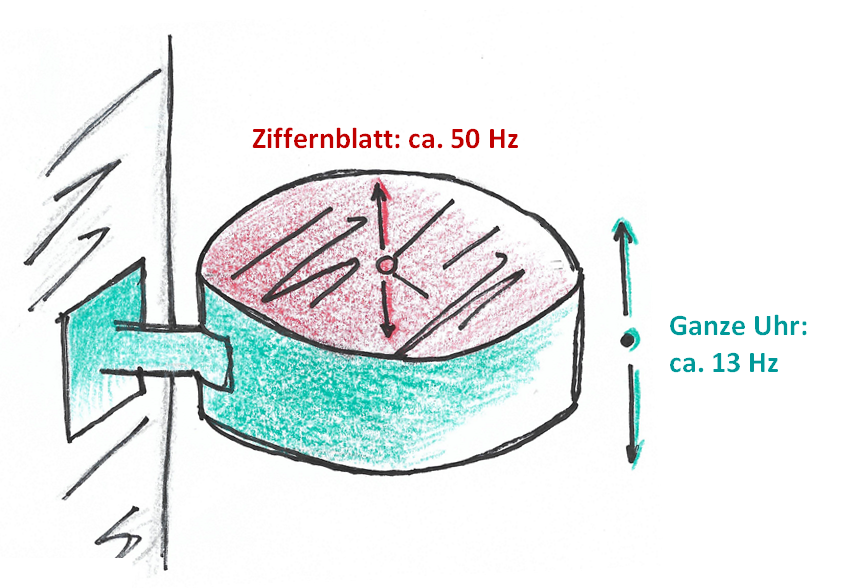
\includegraphics[width=7cm]{img/msg5/frequenzen.png}
			\caption[Darstellung Schwingung der Aussenuhr]{Die beiden stark vertretenen Frequenzen im Spektrum: Ziffernblatt ca. 50Hz, ganze Uhr ca. 13Hz}
			\label{fig:darst_frequ}
		\end{SCfigure}
		Besonders deutlich treten diese oben erw�hnten beiden Frequenzen im Beschleunigungssignal gemessen am Uhrwerk auf. 
		Das Beschleunigungssignal des Sensors am Rahmen aussen weist bei 50Hz einen deutlich kleineren Signalanteil 
		auf. Daf�r ist die Schwigung der ganzen Uhr von ungef�hr 13Hz gut im Spektrum ersichtlich. Das Beschleunigungssignal
		innen an der Uhr ist �ber alle Frequenzen deutlich kleiner als die anderen beiden. 
		\begin{figure}
			\centering
			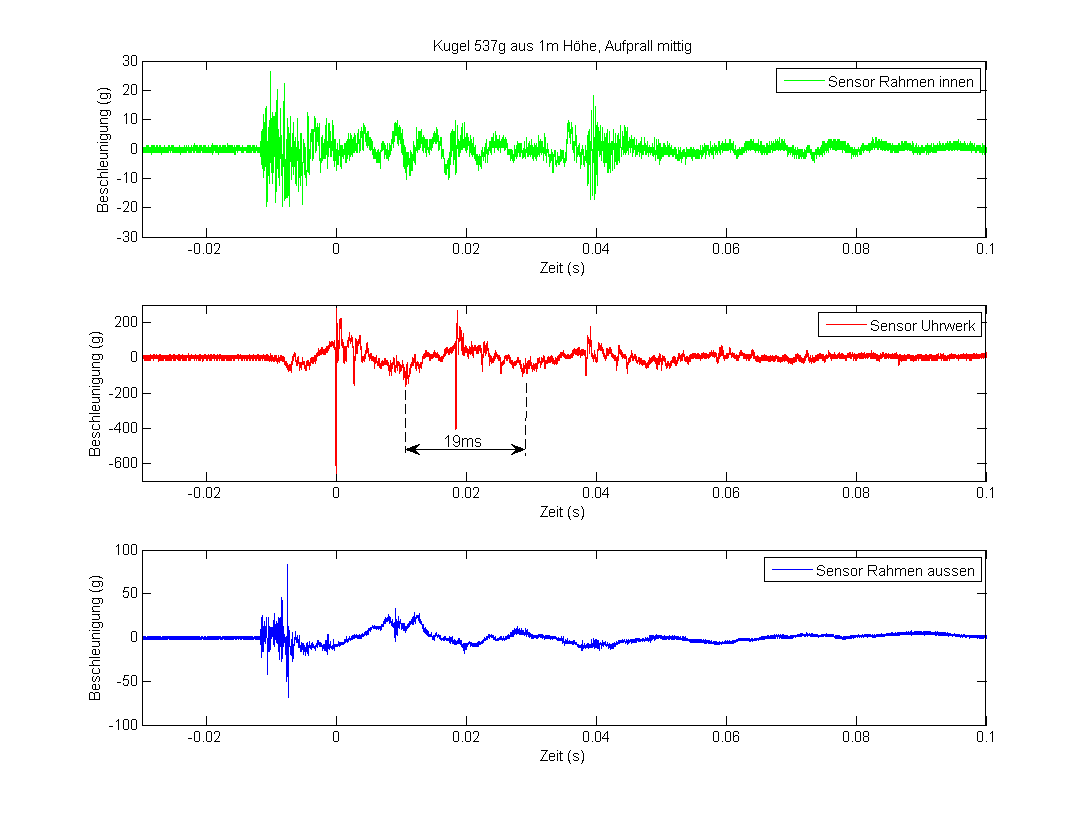
\includegraphics[width=14cm]{img/msg5/max.png}
			\caption[Maximal gemessene Beschleunigungen]{Beschleunigung bei Aufprall einer Stahlkugel mit einer Masse von 537g und aus einem Meter H�he.
%			Gr�n: Sensor Rahmen innen \\
%			Rot: Sensor Uhrwerk \\
%			Blau: Sensor Rahmen aussen	
			}
			\label{fig:max}
		\end{figure}
		\begin{figure}
			\centering
			%\captionsetup{width=15.5cm}
			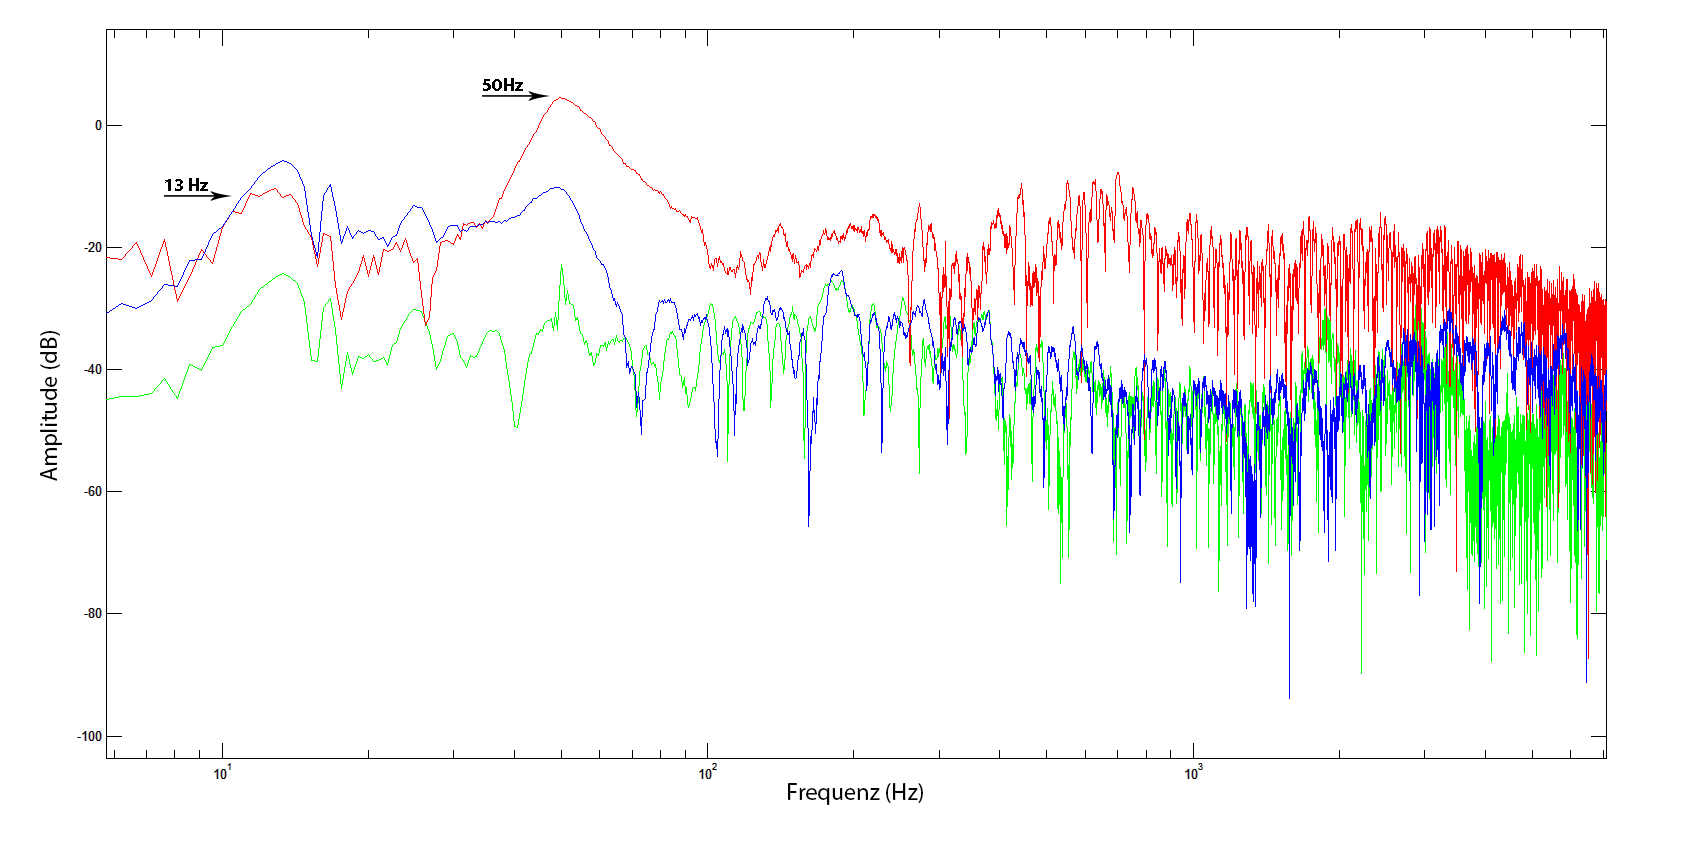
\includegraphics[width=15.5cm]{img/msg5/spektrum.png}
			\caption[Spektren der maximal gemessenen Beschleunigungssignale]{Spektren der Sensoren bei Aufprall einer Stahlkugel mit einer Masse von 537g und aus einem Meter H�he. 
				Gr�n: Spektrum Sensor Rahmen innen.
				Rot: Spektrum Sensor Uhrwerk.
				Blau: Spektrum Sensor Rahmen aussen.
				}
			\label{fig:spect_all}
		\end{figure}
		
		Dies l�sst sich dadurch erkl�ren, dass
		weiter weg von der Befestigung an der Wand die Auslenkung der Uhr gr�sser ist. Da die Periode der
		Schwingung an jedem Punkt dieselbe ist, ist die Geschwindigkeit weiter aussen gr�sser. Daraus
		folgt, dass auch die Beschleunigung an diesem Punkt gr�sser ist.
		
		\begin{SCfigure}
			\centering
			\vspace{-1cm}
			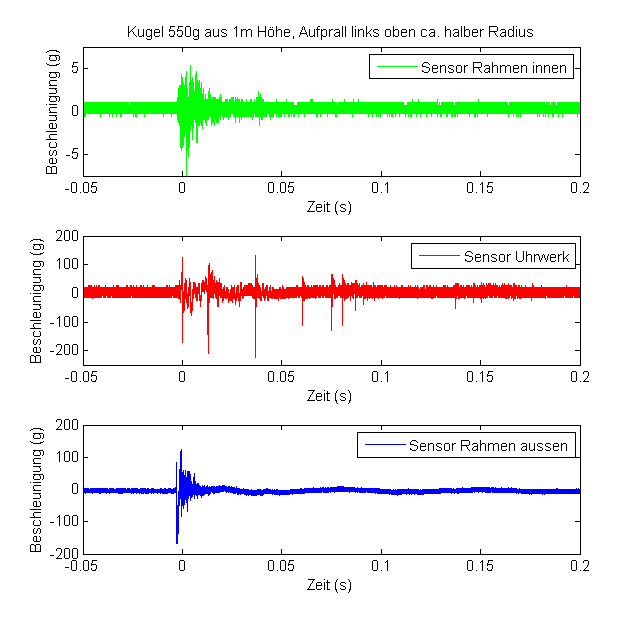
\includegraphics[width=10cm]{img/msg2/break.png}
			\caption[Scheibenbruch]{Beschleunigung bei Aufprall einer Stahlkugel mit einer Masse von 537g und aus zwei Meter H�he. Die Scheibe bricht 
					 in Folge des Aufpralls.}
			\label{fig:bruch}
		\end{SCfigure}
		
		Bei einem Bruch der Scheibe sind die gemessenen Beschleunigungssignale kleiner. Dies ist in
		\autoref{fig:bruch} zu erkennen. Der Stoss ist bei einem Bruch weniger elastisch. Ein Teil der
		kinetischen Energie wird durch die plastische Deformation in innere Energie umgewandelt. Die Kugel
		prallt mit einer kleineren Geschwindigkeit zur�ck als ohne Bruch. Dadurch ist der �bertragene
		Impuls kleiner. Die Folge sind kleinere Beschleunigungen der Uhr. Ein weiterer Grund f�r kleinere
		Beschleunigungssignale ist, dass die Kugel nicht in der Mitte der Scheibe aufgeprallte.
		
		\paragraph{Fazit}
		Durch schwache Schl�ge aus einem Meter H�he lassen sich Beschleunigungssignale gr�sser als 600g am
		Uhrwerk messen. Die Kugel hat beim Aufprall eine Geschwindigkeit $v=\sqrt{2gh} = 4.4 \frac{m}{s}$ und eine Energie 
		$E_{kin}=\frac{1}{2} m v^2 = 5.3J$. Ein Amateur-Handballer erreicht beim Werfen von einem Ball mit einer Masse von ca. 480g aus
		dem Stand Abwurfgeschwindigkeiten von �ber 20 m/s \cite{Gorostiaga}. Die bombierte Scheibe ging
		bereits bei einer Abwurfh�he von 2m und somit einer Aufprallgeschwindigkeit von $6.3\frac{m}{s}$ in die Br�che.
		Es darf somit mit Beschleunigungssignalen im Bereich der dargestellten Messungen gerechnet
		werden.
		
		Im Frequenzspektrum erkennt man zwei Frequenzen, welche besonders stark vertreten sind. Dies ist einerseits
		die Frequenz, mit welcher das Ziffernblatt schwingt, andererseits die Frequenz, mit welcher die ganze Uhr 
		auf- und abschwingt.
	\newpage	
	\section{Ermittlung der besten Sensorposition} \label{subsec:bestPos}
	
		\paragraph{Vorgehensweise}
		Die Position den Sensors an der Aussenuhr ist insofern eingeschr�nkt, dass dieser von aussen nicht 
		sichtbar sein darf. Dies wurde in der Anforderungsliste im Schlussteil \ref{chap:anforderungen} festgehalten. 
		An drei der in Frage kommenden Positionen wurden die piezoelektrischen Sensoren befestigt. 
		Dann wurde die schwerere Stahlkugel mit einer Masse von 537g aus einer H�he von 
		50cm an verschiedenen Stellen auf die Uhr fallen gelassen. Es wurde gleichzeitig mit den drei 
		Beschleunigungssensoren an der Uhr gemessen. Die drei Positionen sind im \autoref{chap:Versuchsaufbau}
		in der \autoref{fig:versuchsaufbau_piezo} ersichtlich:  
		\begin{itemize}
			\item An der Montageleiste der Uhr innen, nahe der Konsole (Channel 1, gr�n)
			\item Am Uhrwerk, welches am Ziffernblatt befestigt ist (Channel 2, rot)
			\item Am Rahmen der Uhr aussen (Channel 3, blau)
		\end{itemize}
		Die Kugel wurde an 4 Positionen der Uhr fallen gelassen: 
		\begin{itemize}
			\item In der Mitte der Scheibe, Resultat Messung \autoref{fig:mittig}
			\item Seitlich an der Scheibe, Resultat Messung \autoref{fig:seitlich}
			\item Aussen auf die Scheibe, Resultat Messung \autoref{fig:aussen}
			\item Innen auf die Scheibe, Resultat Messung \autoref{fig:innen}
		\end{itemize}
		
		\paragraph{Messresultate}
		Die Abbildungen \ref{fig:mittig} bis \ref{fig:innen} zeigen die Messresultate der 4 Messungen mit
		jeweils drei Beschleunigungssignalen aufgezeichnet an der Uhr innen, am Uhrwerk und am Rahmen aussen. 
		Dabei wurden die Achsen bewusst bei allen Messungen gleich
		gross skaliert, damit die Unterschiede der Amplituden gut ersichtlich sind. 
		
		Die gr�ssten Beschleunigungssignale sind am Sensor am Uhrwerk zu messen. Der gemessene Maximalwert erreicht
		mehr als 200g. Die zweitgr�ssten Beschleunigungssignale  sind am Sensor am Rahmen aussen zu messen. Die
		Beschleunigung liegt in einem Bereich bis 100g.  Am Sensor innen sind die kleinsten Ausschl�ge
		messbar. Diese Beschleunigungen �berschreiten maximal 10g. Der Sensor am Uhrwerk detektiert bei
		Aufprallen weiter von der Mitte entfernt kleinere, aber im Vergleich zu den beiden anderen
		Sensoren dennoch grosse Messwerte.
		
		\paragraph{Fazit}
		Unabh�ngig davon, wo die Kugel auf der Scheibe aufprallt, k�nnen am Uhrwerk die gr�ssten
		Beschleunigungssignale gemessen werden. Ein	weiterer Vorteil der Messung am Uhrwerk zeigt sich in
		der Unterscheidung zwischen einem Wurf und einer Druck-Sogwelle eines Zuges in
		\autoref{sec:Unterscheidung}: Im Signal am Uhrwerk ist die Schwingung der ganzen Uhr, aber auch
		die Schwingung des Ziffernblatts erkennbar. Die beste Position f�r den Sensor ist demnach am
		Uhrwerk.
			\begin{figure}[H]
			\hspace{-0.8cm}
				\begin{minipage}[hbt]{8.2cm}
					\centering
					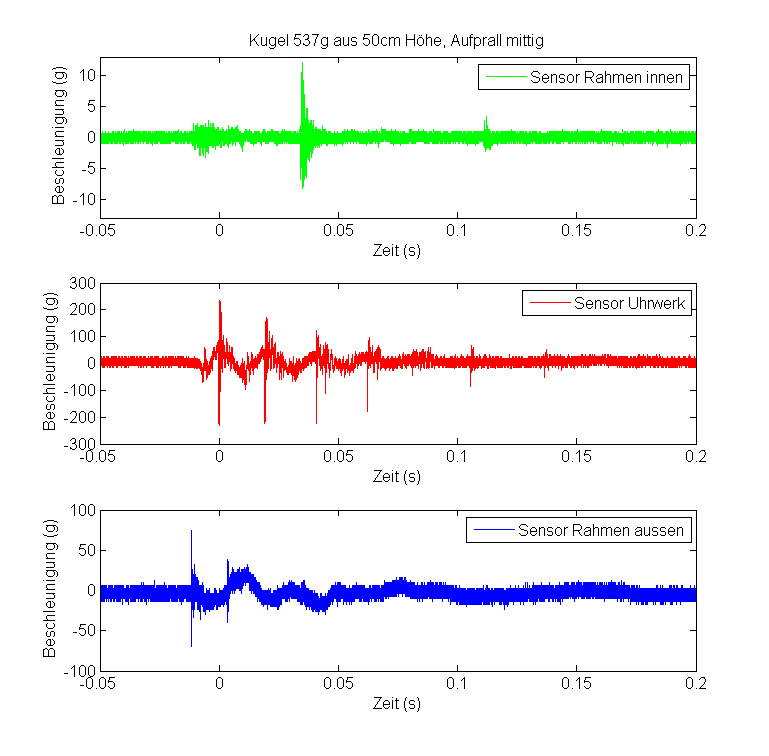
\includegraphics[width=9cm]{img/msg2/mittig.png}
					\vspace{-1cm}
					\caption{Aufprall mittig}
					\label{fig:mittig}
				\end{minipage}
				\hfill
				\begin{minipage}[hbt]{8.2cm}
					\centering
					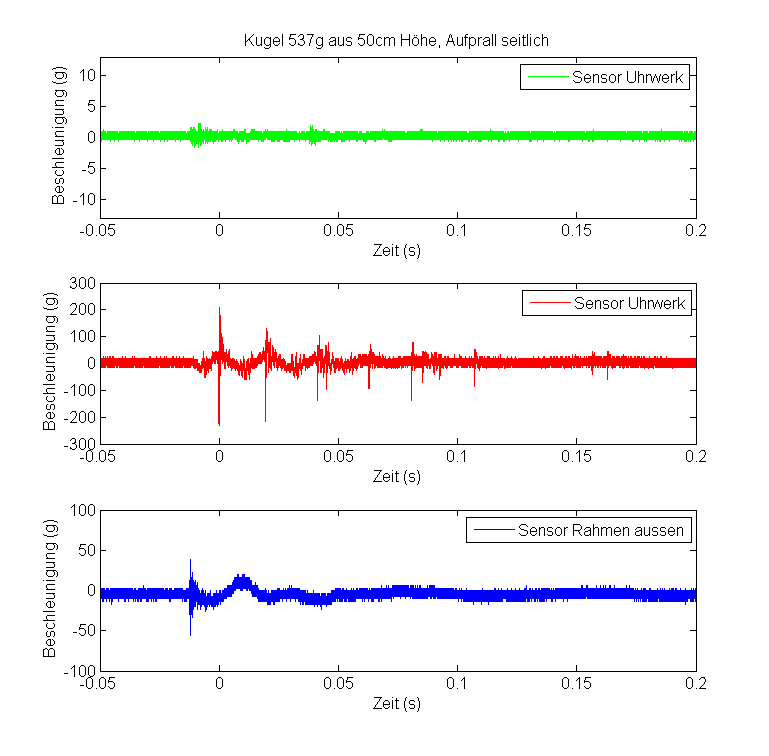
\includegraphics[width=9cm]{img/msg2/seitlich.png}
					\vspace{-1cm}
					\caption{Aufprall seitlich}
					\label{fig:seitlich}
				\end{minipage}
			\end{figure}
			\begin{figure}[H]
				\hspace{-0.8cm}
				\begin{minipage}[hbt]{8.2cm}
					\centering
					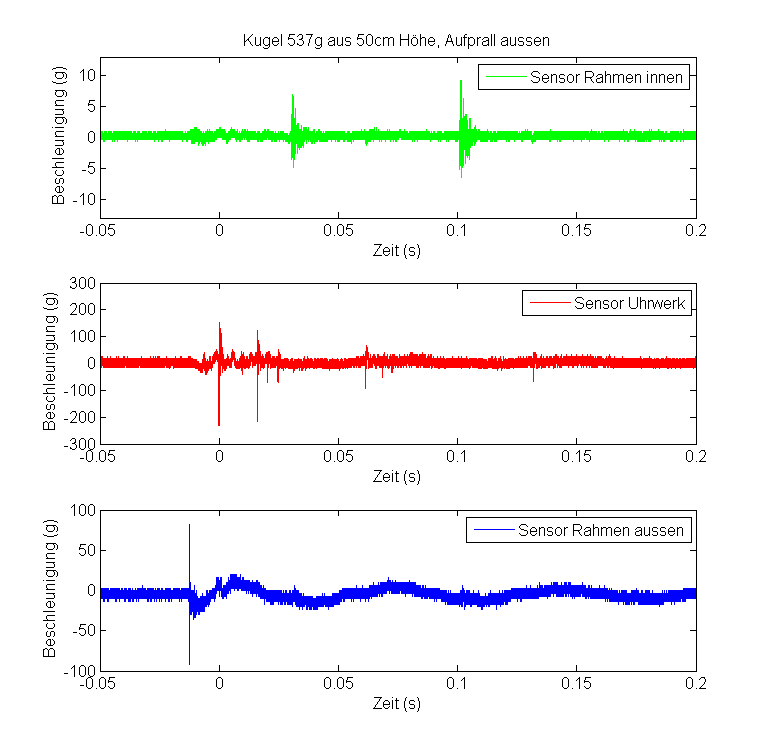
\includegraphics[width=9cm]{img/msg2/aussen.png}
					\vspace{-1cm}
					\caption{Aufprall aussen}
					\label{fig:aussen}
				\end{minipage}
				\hfill
				\begin{minipage}[hbt]{8.2cm}
					\centering
					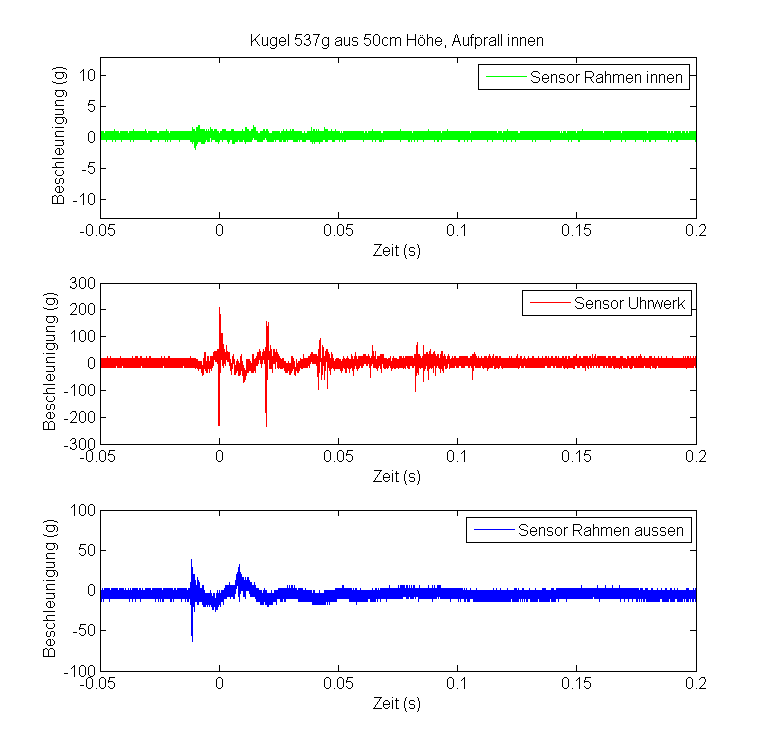
\includegraphics[width=9cm]{img/msg2/innen.png}
					\vspace{-1cm}
					\caption{Aufprall innen}
					\label{fig:innen}
				\end{minipage}
			\end{figure}
	\clearpage	
	\newpage
	\section{Unterscheidung von der Druck-Sogwelle des Zuges} \label{sec:Unterscheidung}
		\paragraph{Vorgehensweise}
			Ein wichtiger Punkt der Machbarkeitsstudie ist es, abzukl�ren, inwiefern die 
			Druck-Sogwelle eines Zuges einen Einfluss auf die Beschleunigung der Aussenuhr hat. 
			Da es sehr zeitaufw�ndig ist, eine Bewilligung f�r Messungen auf Perrons im Fahrleitungsbereich
			zu erhalten, musste eine andere Vorgehensweise gew�hlt werden.
			
			Die auf die Uhr einwirkenden Kr�fte unterscheiden sich bei einem Wurf oder einer Zugdruchfahrt
			prim�r durch folgende Faktoren:
			\begin{itemize}
				\item Gr�sse der Kontaktfl�che
				\item Dauer der Einwirkung
			\end{itemize}
			Aus Differenzdruckmessungen an Fassadenplatten bei der Durchfahrt einer S-Bahn mit
			$v=80\frac{km}{h}$ \cite{diffdruck} ergibt sich eine Dauer von 215ms f�r den Druck-Sog-Wechsel.
			Die dynamische Anregung durch diesen Druck-Sog-Wechsel hat eine Frequenz von 4.65Hz. 
			\begin{figure}[H]
				\centering
				%\captionsetup{width=15.5cm}
				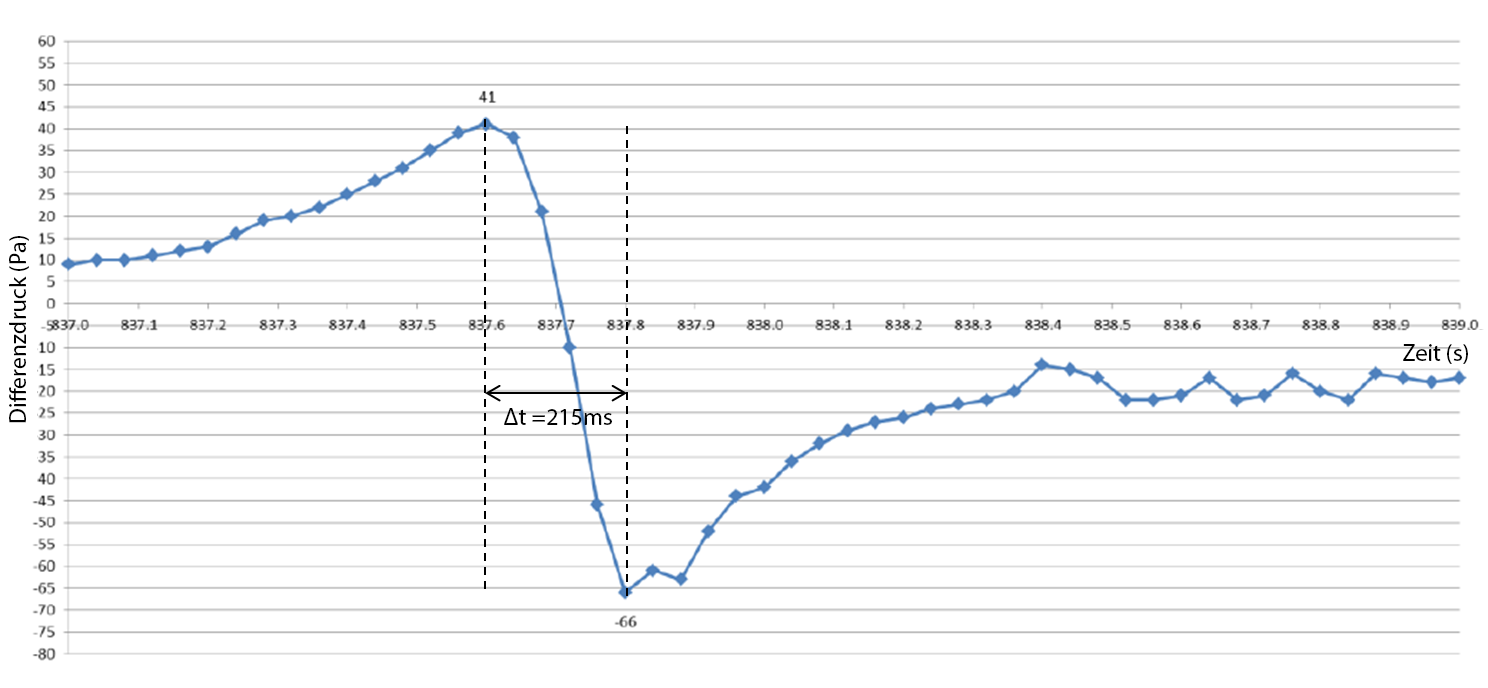
\includegraphics[width=15cm]{img/differenzdruck.png}
				\caption[Differenzdruckmessung]{Differenzdruck gemessen bei Durchfahrt einer S-Bahn mit $v=80\frac{km}{h}$ \cite{diffdruck}. Der Wechsel von Durck zu Sog passiert
					innerhalb von 215ms. Dies entspricht einer Anregung mit einer Frequenz von 4.65Hz.}
				\label{fig:differenzdruck}
			\end{figure}
			Der zeitliche Abstand zwischen Sog-und Druckwelle ist, wie im \autoref{Durck-Sogfeld} aus dem
			Grundlagenteil ersichtlich wird, vom Abstand zum Zug und von der Zuggeschwindigkeit $v$
			abh�ngig. Im erw�hnten Abschnitt ist empirisch ein Zusammenhang zwischen den Gr�ssen Abstand zum
			Zug und Druck-Sog-Abstand hergeleitet worden. Im Worst-Case berechnet mit der
			\autoref{calc:DruckSogAbstand} ergibt sich ein theoretischer zeitlicher Abstand des
			Durck-Sog-Wechsels von 124ms und somit eine dynamische Anregung mit der Frequenz 8Hz. Aus den
			Highspeed Aufnahmen der vorangehenden Versuche konnte die Kontaktzeit der Stahlkugel mit der
			Scheibe ermittelt werden. Sie betr�gt im Mittel ungef�hr 20ms. Die Berechnung und die
			Differenzdruckmessung f�hren zum Schluss, dass durch die gr�ssere Dauer der Einwirkung bei einer
			Zugdurchfahrt sogar im Worst-Case die Aussenuhr als Ganzes und das Ziffernblatt nicht angeregt
			werden, da die Eigenfrequenzen h�her liegen und somit keine Schwingung zustande kommt. Um diese
			�berlegungen zu �berpr�fen, wurden mit der Highspeedkamera Aufnahmen von Bahnhofsuhren bei
			vorbeifahrenden Z�gen gemacht.
		
			Wie in den vorangehenden Versuchen beschrieben, wurde mit zwei verschieden schweren Stahlkugeln
			Messungen gemacht. Um die Krafteinwirkung eines Zuges zu simulieren, wurden zus�tzlich Messungen
			mit einem Softball durchgef�hrt. Dieser hat eine �hnliche Masse (180g) wie die leichtere
			Stahlkugel (256g). Er ist jedoch weich und verformt sich beim Aufprall. Dadurch wird die 
			Kontaktfl�che zwischen Ball und Scheibe gr�sser. Mit dem folgenden Versuch soll der Einfluss
			einer gr�sseren Kontaktfl�che untersucht werden. 
			
		\paragraph{Messresultate}
			Die Aufnahmen mit der Highspeedkamera haben die Vermutungen aus dem obigen Abschnitt best�tigt. 
			Zwei verschiedene Bahnhofsuhren bei zwei vorbeifahrenden Personenz�gen und einem G�terzug zeigten 
			keine sichtbaren Bewegungen. Die Geschwindigkeit der Z�ge betrug wie in den Differenzdruckmessungen \cite{diffdruck}
			ungef�hr 80km/h. Es wurde am Bahnhof Aarburg-Oftringen und Rothrist gemessen. Die Aufnahmen sind 
			auf der CD beigef�gt. 
			
			Die Versuche mit dem Softball haben gezeigt, dass eine gr�ssere Kontaktfl�che beim Aufprall des Softballs
			zu einer um Faktoren kleineren Beschleunigung am Uhrwerk f�hrt. In der
			\autoref{fig:sb_k_time_vergl} sind im oberen Teilbild die Beschleunigungssignale abgebildet,
			welche durch den Aufprall eines Softballs hervorgerufen werden. Sie �bersteigen nie $\pm$6g. Im unteren Teilbild sind die
			Beschleunigungssignale beim Aufprall einer Stahlkugel mit �hnlichem Gewicht dargestellt. Dabei werden 
			ohne weiteres Beschleunigungen gr�sser als $\pm$100g erreicht. Das rote Signal wurde am Uhrwerk, das blaue Signal am Rahmen aussen an der Uhr gemessen.
			\begin{SCfigure}
				\centering
				\vspace{-0.5cm}
				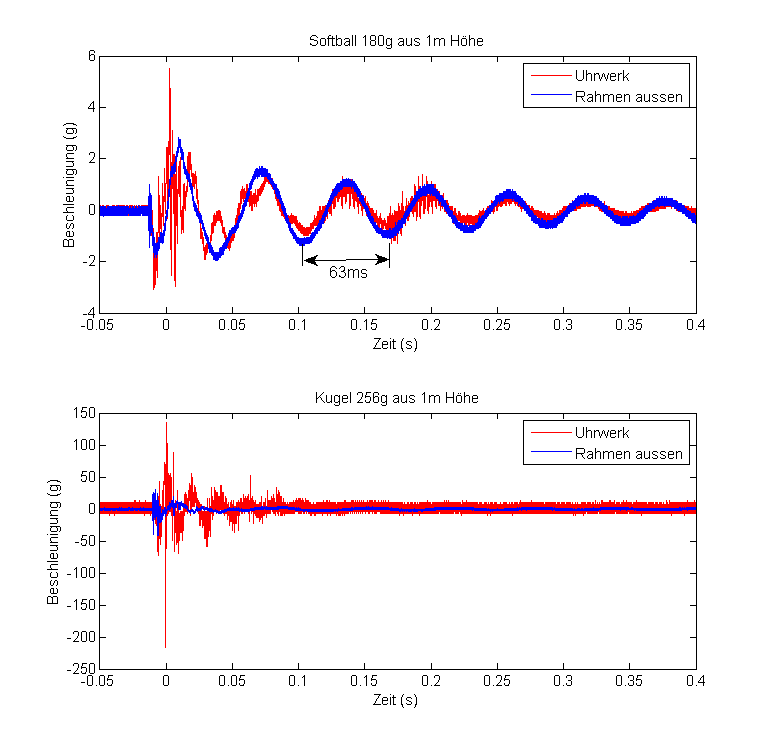
\includegraphics[width=9cm]{img/msg5/vergl_sb_k.png}
				\caption[Vergleich Beschleunigungen Kugel und Softball]{Oberes Teilbild: 
					Softball 180g aus 1m H�he. Unteres Teilbild:\\ 
					Kugel 256g aus 1m H�he.\\\\
					Rot: Sensorsignal Uhrwerk\\
					Blau: Sensorsignal Rahmen aussen}
				\label{fig:sb_k_time_vergl}
			\end{SCfigure} 
			 
			Es f�llt auf, dass beim Aufprall des Softballs die beiden gemessenen Signale am Uhrwerk und am 
			Rahmen aussen die gleiche Frequenz aufweisen. Ausserdem sind die Beschleunigungen beim Aufprall 
			des Softballs am Uhrwerk und am Rahmen aussen �hnlich gross. Die Schwingungsdauer betr�gt 63ms 
			und entspricht einer Frequenz von ungef�hr 16Hz. Daraus ist zu schliessen, 
			in diesem Fall fast ausschliesslich die ganze Uhr schwingt. Das Ziffernblatt wurde nicht angeregt. 
			
			Die am Signal im Zeitbereich beobachteten Eigenschaften k�nnen auch im Frequenzspektrum
			festgestellt werden. Dieses ist in \autoref{fig:spect_vergl} dargestellt. Rot ist das Spektrum
			des Beschleunigungssignals beim Aufprall einer Kugel mit einer Masse von 256g aus einem Meter
			H�he, blau das Spektrum des Beschleunigungssignals beim Aufprall eines Softballs mit einer Masse
			von 180g aus einem Meter H�he, gr�n das Spektrum des Beschleunigungssignals beim Aufprall eines
			Softballs mit einer Masse von 180g aus zwei Metern H�he. Die Kugel und der Ball wurden dabei jeweils
			auf die Mitte der Scheibe fallen gelassen, und das Beschleunigungssignal am Uhrwerk ausgewertet.
			
			Beim Aufprall der Kugel (rot) ist die Frequenz des Ziffernblatt von ca. 50Hz am st�rksten
			vertreten. Diese Frequenz ist um den Faktor 5 st�rker vertreten als die Frequenz der ganzen Uhr
			von ca. 16Hz. Im Gegensatz dazu ist beim Aufprall des Softballs (gr�n) die Frequenz des Ziffernblattes
			um den Faktor 3 schw�cher vertreten als jene der ganzen Uhr. Der Aufprall der Kugel regt somit das
			Ziffernblatt st�rker an als der Softball.  
			
			\begin{figure}
				\centering
				\captionsetup{width=14cm}
				\includegraphics[width=15.5cm]{img/msg5/vergl_sek_sb_k_w.png}
				\caption[Vergleich Spektrum Beschleunigung Aufprall Kugel und Softball]{Spektren der Signale vom Sensor am Uhrwerk: \\\\
					Blau: Spektrum Sensorsignal bei Aufprall des Softballs 188g aus 1m H�he\\
					Rot: Spektrum Sensorsignal bei Aufprall der Kugel 256g aus 1m H�he \\
					Gr�n: Spektrum Sensorsignal bei Aufprall des Softballs 188g aus 2m H�he
					}
				\label{fig:spect_vergl}
			\end{figure}
			
			\paragraph{Fazit}
			
			L�sst man den Softball oder die Stahlkugel aus der gleichen H�he auf die Uhr prallen, haben beide
			Massen beim Aufprall ungef�hr die gleiche kinetische Energie. Die Messungen zeigen jedoch, dass durch den
			Aufprall der Stahlkugel das Ziffernblatt st�rker angeregt wird als durch den Aufprall des
			Softballs.
			
			Aus diesen Beobachtungen folgt die Hypothese, dass der Aufprall eines Mediums auf die Uhr zwei Effekte hat: 
			\begin{itemize}
				\item Verbiegung der ganzen Uhr
				\item Einbuchtung (Deformation) in der Scheibe
			\end{itemize}
			
			Da der Aufprall der Stahlkugel neben der Verbiegung der ganzen Uhr eine Einbuchtung der Scheibe zur Folge hat, 
			wird das Ziffernblatt st�rker angeregt. Diese Anregung wird durch die komprimierte Luft zwischen 
			Scheibe und Ziffernblatt �bertragen. 
			
			Auf der Folgeseite sind je f�nf Bilder aus den Highspeedaufnahmen des Aufpralls der Stahlkugel und 
			des Softballs dargestellt. Der Zeitabstand zwischen den Bildern betr�gt 3 Frames oder umgerechnet 6.25ms. 
			Der Softball wird beim Aufprall zusammengestaucht und hat eine gr�ssere Kontaktfl�che mit der Scheibe als
			die Kugel. In der Scheibe entsteht durch den Aufprall des Softballs keine sichtbare Einbuchtung. Die Luft zwischen 
			Scheibe und Ziffernblatt wird somit weniger komprimiert und das Ziffernblatt weniger angeregt, als es beim Aufprall
			der Kugel der Fall ist. Wie im Abschnitt Vorgehensweise erl�utert wird, greift die auf die Scheibe dr�ckende Luft bei 
			einem vorbeifahrenden Zug auf der ganzen Scheibe gleichm�ssig an. Es ist wahrscheinlich, dass das Ziffernblatt 
			in Folge der Druck-Sogwelle eines Zuges weniger als beim Softball angeregt wird, da die Kontaktfl�che noch gr�sser ist. 
			
			Die \autoref{fig:mod_mfd} zeigt ein Masse-Feder-D�mpfermodell der Aussenuhr. Das Modell wird schnell komplex.
			Bereits dieses stark vereinfachte Modell entspricht einem System 7. Ordnung. Deshalb, und weil die Weiterverfolgung 
			dieses theoretischen Ansatz f�r diese Anwendung nicht zielf�hrend ist, wird das Modell 
			nur benutzt, um die Wege der Kraft�bertragung innerhalb der Uhr zu verdeutlichen: die Kraft greift an der Scheibe an. 
			Sie wirkt einerseits direkt �ber $k_3$ auf den Rahmen der Uhr, andererseits wird durch die komprimierte Luft
			$k_2$ das Ziffernblatt angeregt. 
			
			\begin{figure}
				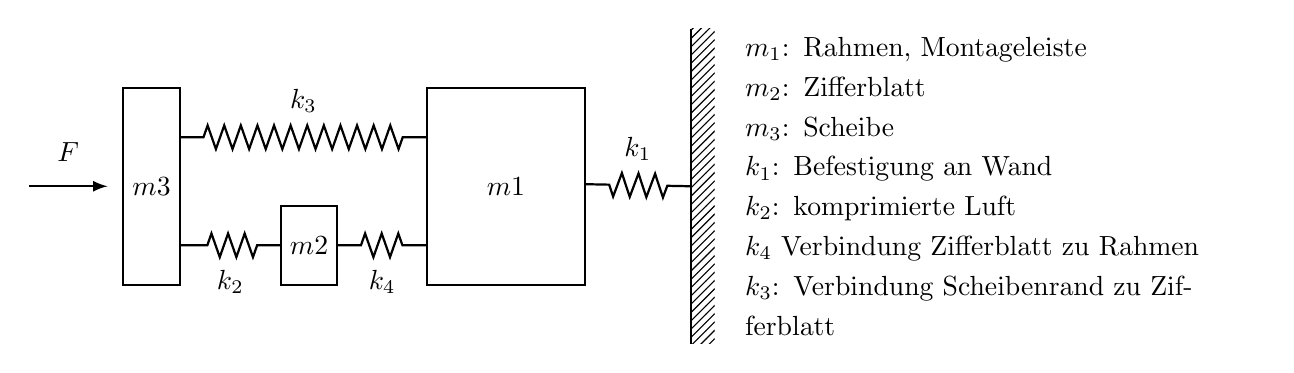
\begin{tikzpicture}[every node/.style={draw,outer sep=0pt,thick}]
				\tikzstyle{spring}=[thick,decorate,decoration={zigzag,pre length=0.3cm,post length=0.3cm,segment length=6,amplitude=1.5mm}]
				\tikzstyle{damper}=[thick,decoration={markings,  
					mark connection node=dmp,
					mark=at position 0.5 with 
					{
						\node (dmp) [thick,inner sep=0pt,transform shape,rotate=-90,minimum width=15pt,minimum height=3pt,draw=none] {};
						\draw [thick] ($(dmp.north east)+(2pt,0)$) -- (dmp.south east) -- (dmp.south west) -- ($(dmp.north west)+(2pt,0)$);
						\draw [thick] ($(dmp.north)+(0,-5pt)$) -- ($(dmp.north)+(0,5pt)$);
					}
				}, decorate]
				\tikzstyle{ground}=[fill,pattern=north east lines,draw=none,minimum width=1cm,minimum height=0.3cm]
				
				\node (M1) [minimum width=2cm, minimum height=2.5cm,draw,outer sep=0pt,thick] {$m1$};				% Masse 1
				
				\node (wall) [ground, rotate=-90, minimum width=4cm,yshift=2.5cm] {};								% Mauer
				\draw[thick] (wall.south east) -- (wall.south west);												% Strich an Mauer
				
				\draw [spring] (wall.south) -- node[above=2mm,draw=none]{$k_1$}($(M1.south east)!(wall.100)!(M1.north east)$);	% Befestigung Mauer
				
				\node (M2) [minimum width=0.5cm, minimum height =1cm,yshift=-0.75cm, xshift=-2.5cm] {$m2$};
				\draw [spring](M2.east) -- node[below=2mm,draw=none]{$k_4$} ($(M1.north west)!(M2.west)!(M1.south west)$);		% 
				
				\node (M3) [minimum width=0.5cm, minimum height =2.5cm,yshift=0cm, xshift=-4.5cm] {$m3$};
				\draw [spring] (M2.west) -- node[below=2mm,draw=none]{$k_2$}($(M3.north east)!(M2.east)!(M3.south east)$);		% Komprimierte Luft
				\draw [spring] (M3.60) -- node[above=2mm,draw=none]{$k_3$}($(M1.north west)!(M3.60)!(M1.south west)$);
				
				
				\draw [latex-, thick] (M3.west) ++ (-0.2cm,0) --node[above=2mm,draw=none]{$F$} +(-1cm,0);
				\node [rectangle,text width=6.5cm,align=left, draw=none] at ( $ (current bounding box.center) + (8,0) $ ) {$m_1$: Rahmen, Montageleiste\\ $m_2$: Zifferblatt \\$m_3$: Scheibe \\ $k_1$: Befestigung an Wand\\ $k_2$: komprimierte Luft\\ $k_4$ Verbindung Zifferblatt zu Rahmen \\ $k_3$: Verbindung Scheibenrand zu Zifferblatt} ;		
				\end{tikzpicture}
				\caption{Masse-Feder-D�mpfermodell}
				\label{fig:mod_mfd}
			\end{figure}
			\newpage
			\begin{SCfigure}[]
				\begin{minipage}[hbt]{5cm}
					\centering
					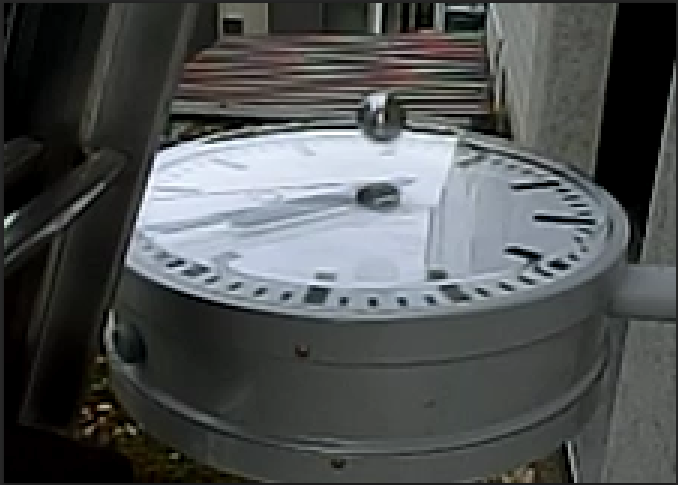
\includegraphics[width=5cm]{img/aufprallVergl/K1.png}
					\vspace{-1cm}
					%\caption{Aufprall mittig}
					%\label{fig:mittig}
				\end{minipage}
				\hfill
				\begin{minipage}[hbt]{5cm}
					\centering
					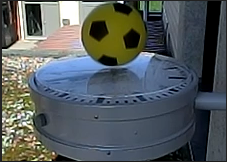
\includegraphics[width=5cm]{img/aufprallVergl/B1.png}
					\vspace{-1cm}
					%\caption{Aufprall seitlich}
					%\label{fig:seitlich}
				\end{minipage}
			\end{SCfigure}
			\begin{SCfigure}[]
				\begin{minipage}[hbt]{5cm}
					\centering
					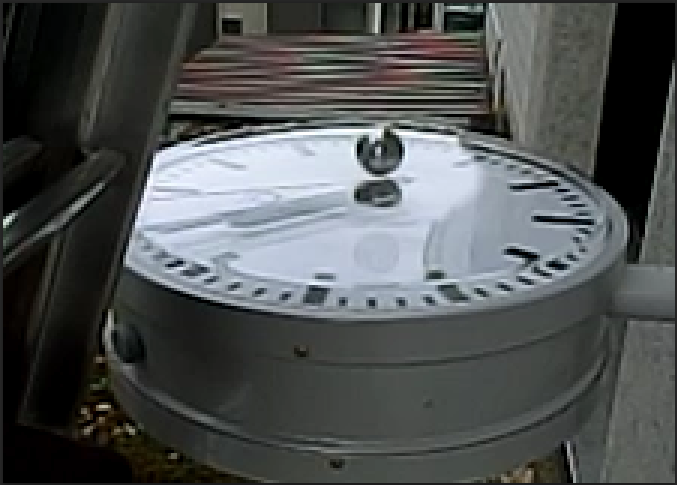
\includegraphics[width=5cm]{img/aufprallVergl/K2.png}
					\vspace{-1cm}
					%\caption{Aufprall mittig}
					%\label{fig:mittig}
				\end{minipage}
				\hfill
				\begin{minipage}[hbt]{5cm}
					\centering
					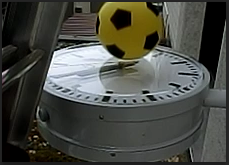
\includegraphics[width=5cm]{img/aufprallVergl/B2.png}
					\vspace{-1cm}
					%\caption{Aufprall seitlich}
					%\label{fig:seitlich}
				\end{minipage}
			\end{SCfigure}
			\begin{SCfigure}[]
				\begin{minipage}[hbt]{5cm}
					\centering
					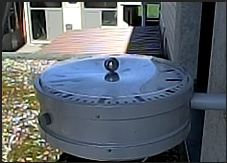
\includegraphics[width=5cm]{img/aufprallVergl/K3.png}
					\vspace{-1cm}
					%\caption{Aufprall mittig}
					%\label{fig:mittig}
				\end{minipage}
				\hfill
				\begin{minipage}[hbt]{5cm}
					\centering
					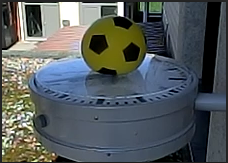
\includegraphics[width=5cm]{img/aufprallVergl/B3.png}
					\vspace{-1cm}
					%\caption{Aufprall seitlich}
					%\label{fig:seitlich}
				\end{minipage}	
			\end{SCfigure}
			\begin{SCfigure}[]
				\begin{minipage}[hbt]{5cm}
					\centering
					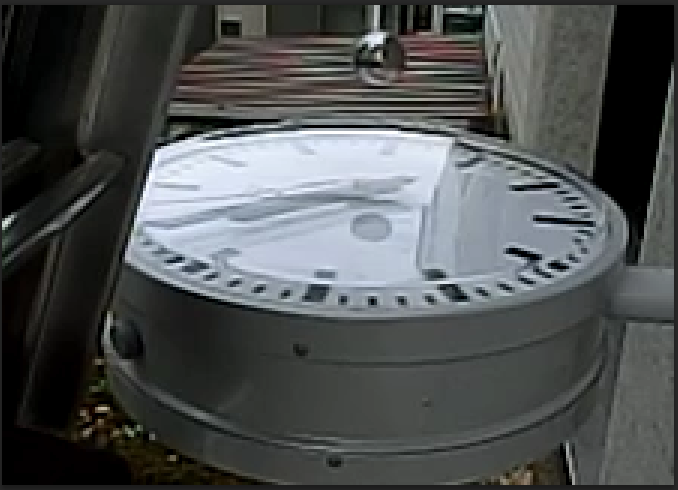
\includegraphics[width=5cm]{img/aufprallVergl/K4.png}
					\vspace{-1cm}
					%\caption{Aufprall mittig}
					%\label{fig:mittig}
				\end{minipage}
				\hfill
				\begin{minipage}[hbt]{5cm}
					\centering
					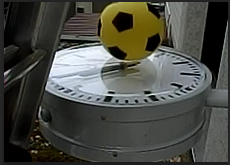
\includegraphics[width=5cm]{img/aufprallVergl/B4.png}
					\vspace{-1cm}
					%\caption{Aufprall seitlich}
					%\label{fig:seitlich}
				\end{minipage}	
			\end{SCfigure}		
			\begin{SCfigure}[]
				\begin{minipage}[hbt]{5cm}
					\centering
					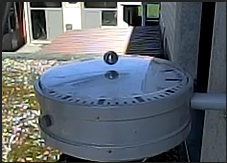
\includegraphics[width=5cm]{img/aufprallVergl/K5.png}
					\vspace{-1cm}
					%\caption{Aufprall mittig}
					%\label{fig:mittig}
				\end{minipage}
				\hfill
				\begin{minipage}[hbt]{5cm}
					\centering
					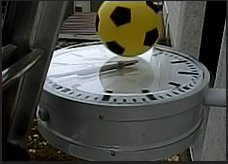
\includegraphics[width=5cm]{img/aufprallVergl/B5.png}
					\vspace{-1cm}
					%\caption{Aufprall seitlich}
					%\label{fig:seitlich}
				\end{minipage}	
			\end{SCfigure}
		Die Einbuchtung der Scheibe durch die Kugel ist besonders gut an der Schattenlinie im Bild erkennbar. Die Kante des Schattens verformt sich beim Aufprall 
		der Kugel, beim Softball sieht man keine Ver�nderung.
		 
		
		
	
		
	
\chapter{Versuche mit dem MEMS Sensor Datenlogger} 
	In einem weiteren Schritt wird der MEMS Beschleunigungssensor H3LIS331DL von STMicroelectronics 
	in einer Datenloggeranwendung in Betrieb genommen werden. Auch die pinkompatiblen und etwas 
	g�nstigeren Beschleunigungssensoren der gleichen Produktreihe eignen sich bestens f�r das Endprodukt. 
	
	\section{Hardware} 
				\begin{wrapfigure}[10]{r}{4cm}
					%\centering
					%\captionsetup{width=4cm}
					\vspace{-1cm}
					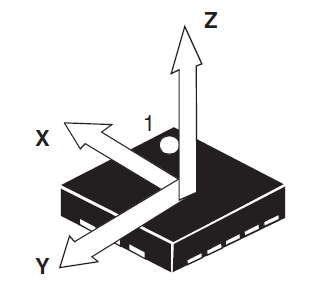
\includegraphics[width=4cm]{img/mems_axes.png}
					\caption[Achsen des H3LIS331DL]{Achsen des H3LIS331DL aus \cite{H3L}}
					\label{fig:mems_axes}
				\end{wrapfigure}
		Die Versuche mit den piezoelektrischen Sensoren in \autoref{subsec:signale} haben gezeigt, dass
		Beschleunigungen �ber 100g gemessen werden. Deshalb wurde besonders auf einen grossen
		Dynamikbereich geachtet. Ausserdem muss die Abtastfrequenz �ber 100Hz liegen. Es wurde der Sensor
		H3LIS331DL von STMicroelectronics eingesetzt. Dieser hat einen einstellbaren Bereich von $\pm100g$,
		$\pm200g$ und $\pm400g$. Die Daten werden digitalisiert. Es kann �ber I2C
			\footnote{engl. \emph{Inter-Integrated Circuit}. I2C ist ein serieller Datenbus. Es	\index{SPI} \index{I2C}
				werden zwei Leitungen verwendet, Clock (SCL) und Daten (SDA) } 
		oder SPI 
			\footnote{engl. \emph{Serial Peripheral Interface}. SPI ist ebenfalls ein serieller Datenbus, 	
				dabei werden vier Leitungen verwendet: Clock (SCLK), Master Output Slave Input (MOSI), 
				Master Input Slave Output (MISO) und Chip Select (CS). }
		mit dem Sensor kommuniziert werden. Die Abtastfrequenz kann zwischen 0.5Hz bis 1kHz konfiguriert
		werden. Der Sensor ist mit der Gr�sse von 3x3x1mm$^2$ sehr klein. Zwei Interruptausg�nge k�nnen
		konfiguriert werden. Eine M�glichkeit ist beispielsweise, dass ein �berschreiten eines Schwellwerts
		angezeigt wird. Weitere Eigenschaften des Sensors k�nnen dem Datenblatt \cite{H3L} entnommen
		werden. Als zweite Komponente wurde ein FRDM-K64F Freedom Board verwendet. Dieses bietet neben der
		Konfiguration des Sensors die M�glichkeit, die ausgelesenen Daten auf einer SD-Karte zu speichern.
		Mit einer Power Bank kann das Freedom Board und der Sensor gespeist werden. So bleibt die
		Messeinheit mobil. In der \autoref{fig:mems_aufbau} sind die drei Komponenten des Aufbaus
		dargestellt.
		%\begin{wrapfigure}[11]{r}{5.5cm}

		\begin{figure}
			\centering
			%\vspace{-1cm}
			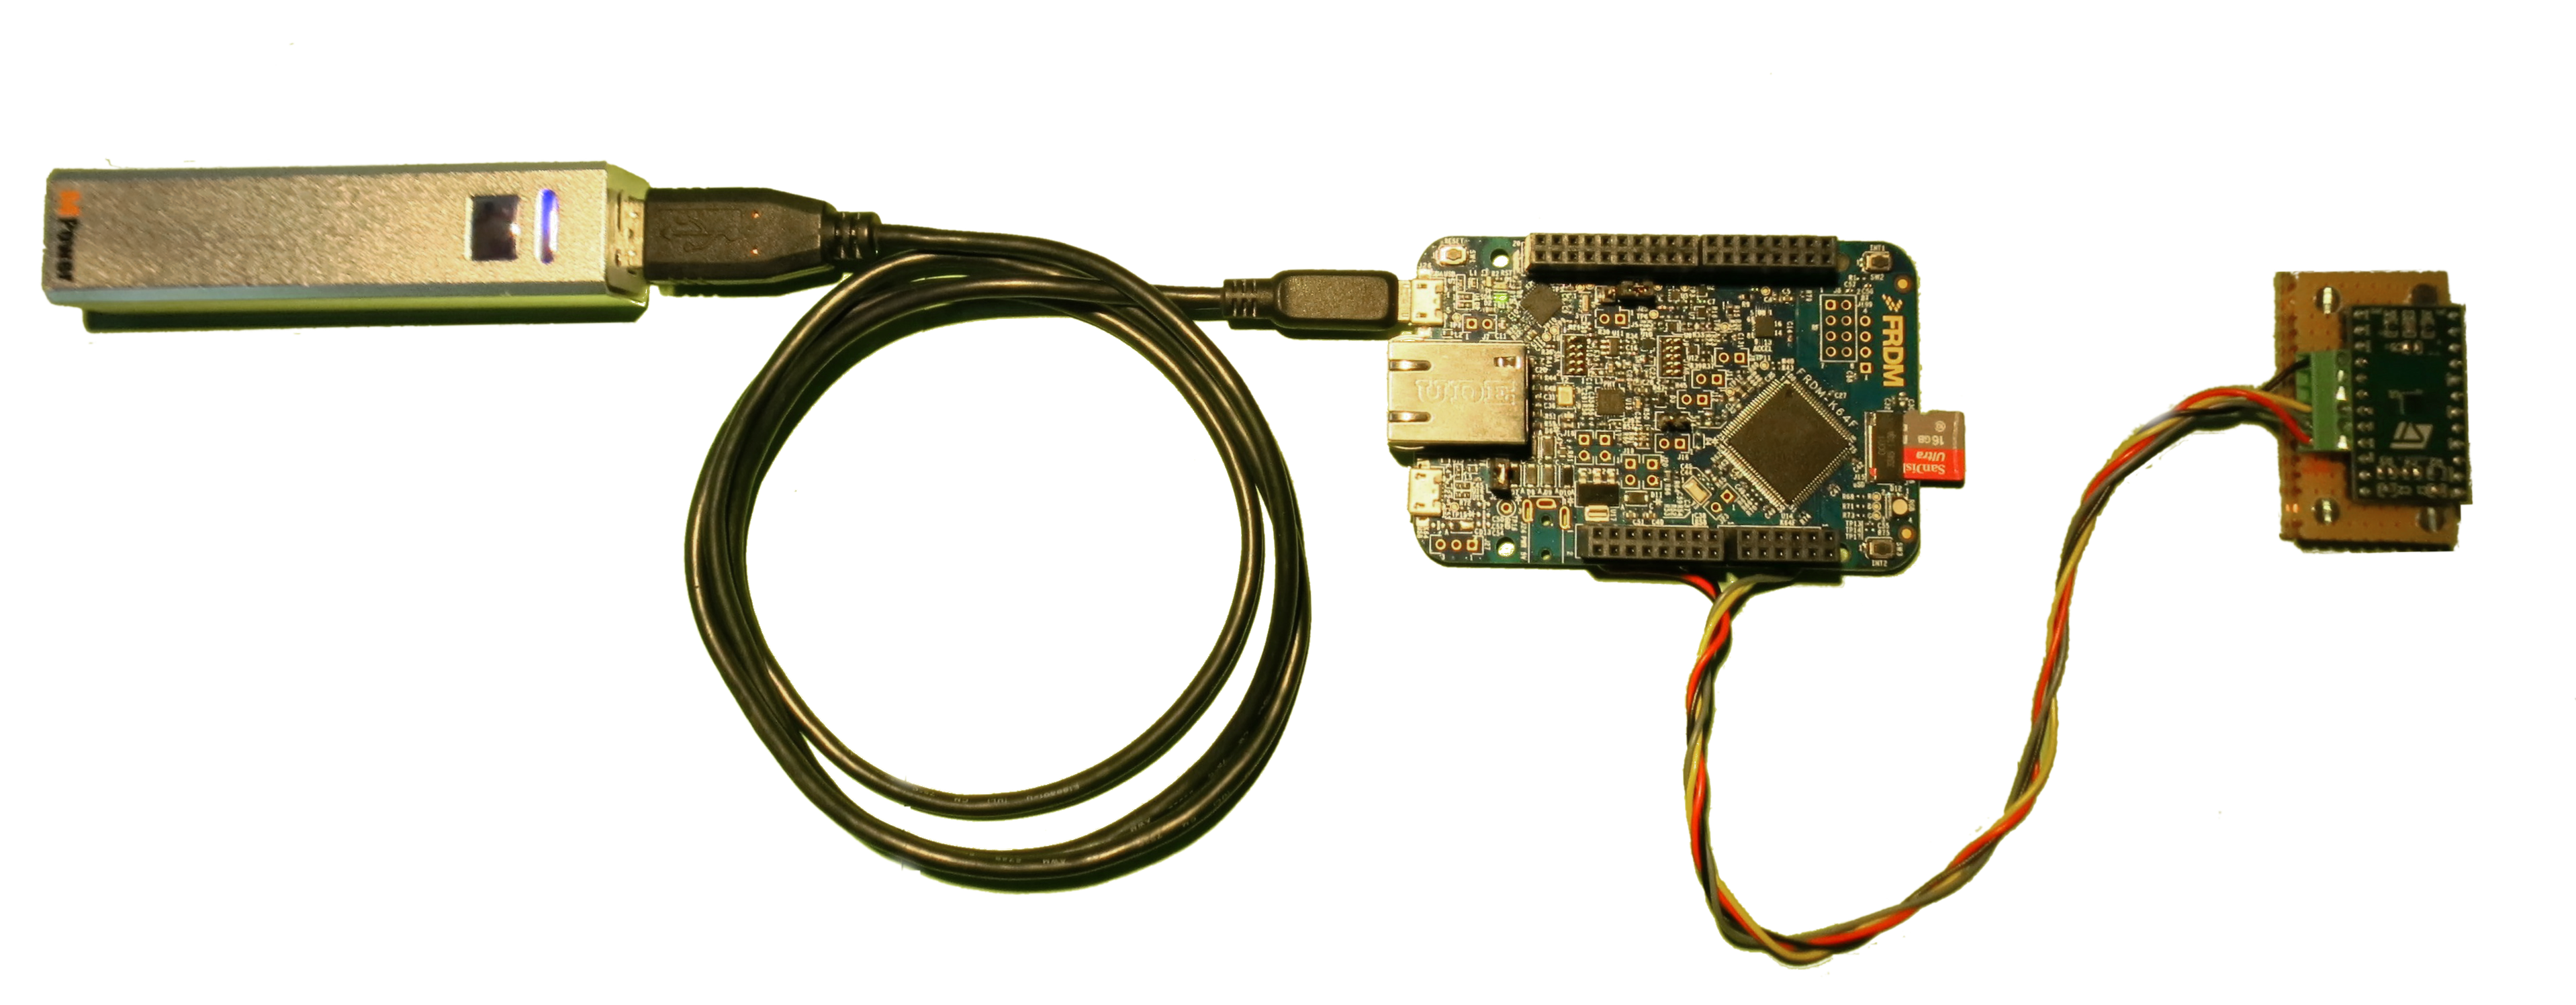
\includegraphics[width=15cm]{img/mems_aufbau.png}
			\caption[Aufbau Datenlogger]{Der Aufbau mit Power Bank, Freedom Board und MEMS-Sensor}
			\label{fig:mems_aufbau}
		\end{figure}
	
	\section{Logging Software}
		F�r die Software wurde FreeRTOS pr�emptiv verwendet. Die Software ist in vier Tasks aufgebaut. Der
		Idle-Task wird immer dann ausgef�hrt, wenn kein anderer Task die CPU ben�tigt. Dieser wird
		automatisch kreiert. Der Main-Task hat die Aufgabe, die Tasten zu pollen und die Events zu handeln.
		Wichtiger f�r den Aufbau der Software ist der Sensor-Task und der SD-Karten-Task. Der Sensor-Task
		kommuniziert �ber I2C mit dem Sensor und liest Daten, falls vorhanden, vom Sensor aus. Er speichert
		ausserdem diese Daten in einer Queue
			\footnote{Eine Liste mit Eintr�gen, welche abgearbeitet werden sollen. Eine Queue kann
				einen Aufrufer blockieren, falls sie voll oder leer ist. }.
		Der SD-Karten-Task wiederum liest die Daten aus der
		Queue, speichert diese in einem Buffer als String. Ist der Buffer voll, wird dieser auf die
		SD-Karte gespeichert. Der Grund dieser Aufteilung ist, dass der Zugriff auf die SD-Karte lange
		dauern kann. Wird jeder Beschleunigungswert einzeln auf die SD-Karte geschrieben, kann nicht mit
		400Hz abgetastet werden. Die Software kann den Sensor nicht genug schnell auslesen und die
		Beschleunigungsdaten werden im Datenregister des Sensors �berschrieben. Werden die
		Beschleunigungsdaten jedoch in einem Buffer gespeichert und dieser als Ganzes auf die SD-Karte
		geschrieben, ist dies effizienter und die Abtastung mit 400Hz m�glich.
		
		Im Sensor-Task und im SD-Karten-Task werden Zustandsautomaten durchgearbeitet. Diese k�nnen einerseits
		durch Tastendr�cke oder Interne Signale beeinflusst werden. Die Kommunikation zwischen dem Main-Task,
		dem Sensor-Task und dem SD-Karten-Task erfolgt dabei mittels Task Notifications. 
		
		Task Notifications gibt es ab FreeRTOS V8.2.0 (Release 16. Januar 2015). Sie dienen der
		Inter-Task-Kommunikation und Synchronisation, �hnlich den Semaphoren. Jeder Task hat dabei einen
		32-bit Notification Value. Jedes dieser Bits des Notification Values kann von einem anderen Task
		gesetzt, �berschrieben oder inkrementiert werden. Es k�nnen auch mehrere Bits gleichzeitig
		modifiziert werden. Task Notifications sind effizienter als Semaphoren \cite{TaskNotification}.
		
		In dieser Anwendung wurde jeweils ein Bit des Notification Values einem Tastendruck oder einem
		internen Signal zugewiesen. Der Main-Task setzt beispielsweise bei einem Tastendruck des Buttons 2
		das erste Bit BTN2\_BIT im Notification Value des Sensor-Tasks. Der Sensor-Task wechselt seinen
		Zustand von "'IDLE"' in "'MEASURE"', wenn dieses Bit gesetzt wurde.
	
		Die \autoref{fig:sm_sensor} und \autoref{fig:sm_sd} veranschaulichen die beiden Zustandsautomaten im 
		Sensor-Task und SD-Karten-Task. 
		\begin{figure}
			\centering
			%\vspace{-1cm}
			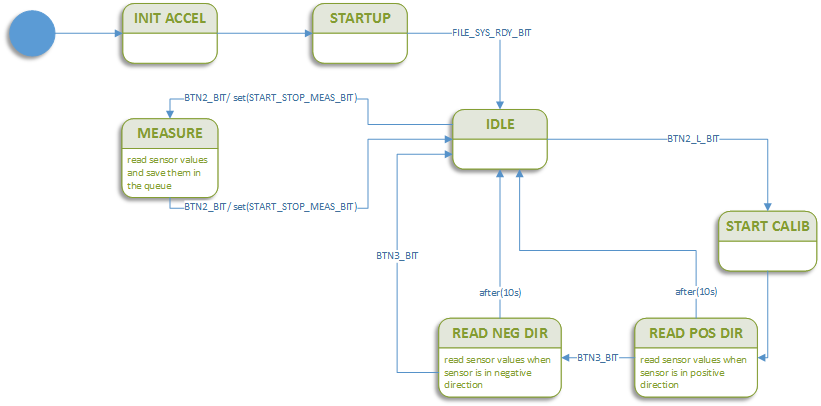
\includegraphics[width=15cm]{img/sm_sensor.png}
			\caption{Zustandsdiagramm Sensor-Task}
			\label{fig:sm_sensor}
		\end{figure}
		
		\paragraph{Sensor-Task}
		Der Zustandsautomat durchl�uft den Zustand "'INIT ACCEL"' in welchem der Sensor konfiguriert 
		wird. Zuerst wird getestet, ob der Sensor antwortet. Dann werden der Messbereich, die Abtastrate, 
		der Power-Modus und die Art der Datenaufbereitung eingestellt. Der Sensor kann im Normal Powermodus
		betrieben werden, oder aber in verschiedenen Low Powermoden. In den Low Powermoden ist die 
		Abtastrate nicht konfigurierbar und tiefer als im Normal Powermodus. 
		
		Nachdem der Sensor konfiguriert ist, wechselt der Zustandsautomat in den Zustand "'STARTUP"'. Hier wird
		so lange gewartet, bis der SD-Karten-Task mit einer Task Notification bekannt gibt, dass er das File 
		System gemountet hat und dieses nun verf�gbar ist. Dann wird der Zustand "'IDLE"' erreicht.
		
		Hier sind zwei Optionen m�glich. Ein Tastendruck des Buttons 2 startet die Messung. Dabei wird
		an den SD-Karten-Task eine Task Notification gesendet, dass die Messung begonnen hat. Der 
		Zustandsautomat verl�sst den Zustand "'MEASURE"' erst dann, wenn der Button 2 erneut gedr�ckt 
		wird. 
		
		Die zweite Option ist die Kalibrierung des Sensors. Dazu muss der Button 2 l�nger als eine Sekunde gedr�ckt
		werden. Mit einem roten Blinken wird der Kalibriermodus dem Benutzer best�tigt. Der Sensor 
		muss nach oben gerichtet werden. Ein Tastendruck des Buttons 3 l�st dann eine Messreihe von 10 
		Messungen aus, �ber die gemittelt wird. Nun muss der Sensor nach unten gerichtet werden und 
		erneut mit einem Tastendruck des Buttons 3 best�tigt werden. Nun wiederholt sich die Messreihe. 
		Jetzt wird der Beschleunigungswert gemessen in Ausrichtung nach unten dem Beschleunigungswert
		gemessen nach oben abgezogen und mit zwei dividiert. So erh�lt man den Wert, der einer Beschleunigung
		von 1g entspricht. Wird der Button 3 jeweils nicht innerhalb von 60s gedr�ckt, wechselt der Zustand zur�ck zu "'IDLE"'.
		
		\paragraph{SD-Karten-Task}
		Der Zustandsautomat durchl�uft zu Beginn den Zustand "'STARTUP"', in welchem das File System gemountet 
		wird. Nachdem dies gelungen ist, wird eine Task Notification an den Sensor-Task gesendet und in den 
		Zustand "'IDLE"` gewechselt. 
		
		Dieser Zustand wird verlassen, falls die Messung gestartet wurde und dies dem SD-Karten-Task durch eine 
		Task Notification vom Sensor-Task mitgeteilt wird. Der Zustandsautomat erreicht den Zustand "'OPEN FILE"'
		in welchem entweder ein bereits vorhandenes Text Dokument ge�ffnet oder sonst ein neues angelegt. Danach 
		wird in den Zustand "'Buffer"' gewechselt. 
		
		In diesem werden die Beschleunigungsdaten aus der Queue gelesen und mit Carriage Return und Line Feed
		Steuerzeichen erg�nzt in einen Buffer gespeichert. Ist der Buffer voll, wird in den n�chsten 
		Zustand gewechselt, ansonsten werden die Beschleunigungsdaten weiter ausgelesen und in den 
		Buffer abgef�llt. 
		
		Im Zustand "'SAVE ON DISK"' wird der volle Buffer auf die SD-Karte geschrieben. Dann wird erneut in 
		den Zustand "'BUFFER"' gewechselt. Dies wiederholt sich so lange, bis der Sensor-Task mittels
		einer Task Notification das Ende der Messung anzeigt. 
		\begin{figure}
			\centering
			%\vspace{-1cm}
			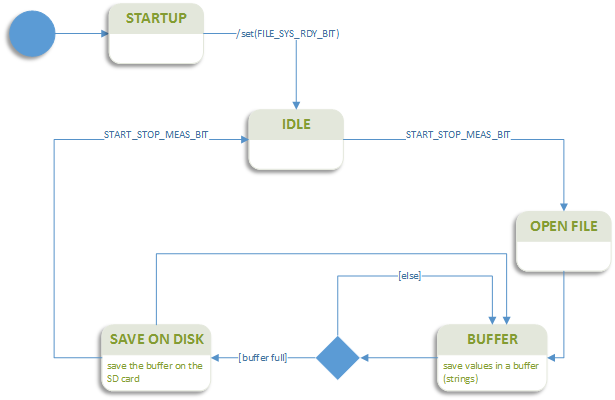
\includegraphics[width=13cm]{img/sm_sd.png}
			\caption{Zustandsdiagramm SD-Karten-Task}
			\label{fig:sm_sd}
		\end{figure}
		\vspace{-1.2cm}
		\paragraph{Sensor Treiber}
		Mittels I2C oder SPI kann auf die Register des Sensors H3LIS331DL zugegriffen werden. Die Register
		dienen einerseits der Konfiguration des Sensors, anderseits um die Beschleunigungsdaten und 
		den Status des Sensors auszulesen. F�r die Datenloggeranwendung wurde ein Treiber erstellt. Dieser
		enth�lt Funktionen, um die Sensor internen Register zu beschreiben oder auszulesen. Hier soll an zwei Beispielen 
		gezeigt werden, wie die Treiberfunktionen aufgebaut sind. 
		Beim ersten Beispiel soll der Messbereich des Sensors konfiguriert werden. Einstellbar sind
		$\pm100g$, $\pm200g$ und $\pm400g$. Dies kann mittels beschreiben der Bits 4 (FS0) und 5 (FS1) des
		Kontrollregisters CTRL\_REG4 erreicht werden. Dieses Register wird �ber die Registeradresse 0x23
		angesprochen. 
		
		\begin{figure}
			\centering
			%\vspace{-1cm}
			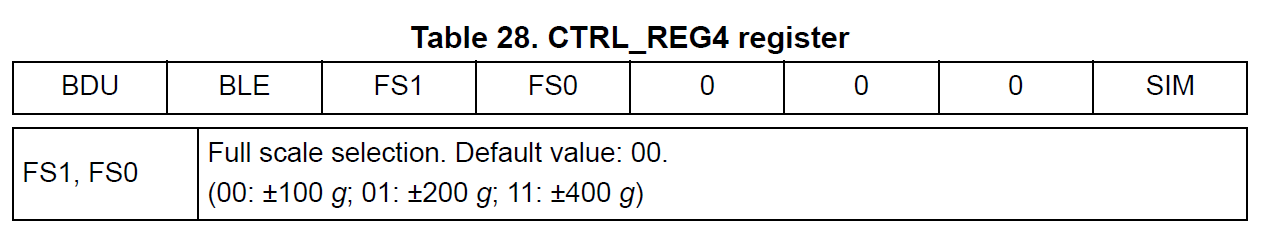
\includegraphics[width=13cm]{img/kontrollregister.png}
			\caption[Kontrollregister 4 des H3LIS331DL]{Kontrollregister 4, Ausschnitt aus dem Datenblatt des H3LIS331DL \cite{H3L}}
			\label{fig:sm_sd}
		\end{figure}
	
		Damit die anderen Bits des Registers nicht f�lschlicherweise �berschrieben werden, wird das Register zuerst ausgelesen (Zeile 6). 
		Nach jedem Lese- oder Schreibzugriff wird gepr�ft, ob dieser erfolgreich verlief (Zeile 7-9). Die nicht
		zu beschreibenden Bits werden ausmaskiert (Zeile 10). Der der Funktion als Parameter �bergebene Wert
		rg muss nun noch nach links geschoben werden. Bit 4 und 5 werden nun beschrieben (Zeile 11). 
		Zuletzt muss der neue Wert f�r das Kontrollregister an den Sensor gesendet werden (Zeile 14). 
		
		\lstset{language=C}
		\lstinputlisting{code/setRange.c}
		
		Im zweiten Beispiel werden die Beschleunigungsdaten f�r die Z-Richtung ausgelesen. Die Daten werden 
		in zwei Registern gespeichert. Sie sind als Zweierkomplement dargestellt. Ein Beschleunigungswert
		ist 12 Bit lang. Dieser wird linksb�ndig gespeichert. 
		
		\lstinputlisting{code/getRawData.c}
		
		Wenn man mehr als ein Register auf einmal auslesen will, kann man das in der Registeradresse 
		signalisieren, indem man das MSB \footnote{engl. \emph{most significant bit}. Hier Bit 7.} auf
		eins setzt. Zus�tzlich muss angegeben werden, wie viele Register ausgelesen werden sollen (Zeile 1 \& 6). 
		
		Damit die Daten richtig interpretiert werden, m�ssen die ausgelesenen Register zuerst in einem 
		unsigned Typ gespeichert werden. Dann wird das High Byte um 8 Stellen nach links geschoben und in einem 
		unsigned Typ gespeichert. Jetzt m�ssen die beiden Register durch eine bitweise Oder-Verkn�pfung
		zusammengef�hrt werden (Zeile 10). Der so interpretierte Wert ist nun, da nur 12 Bit lang, eigentlich um den 
		Faktor 16 zu gross. Dieser Faktor kann beispielsweise in die Umrechnung in m/s$^2$ integriert 
		werden. 
	\newpage
	\section{Versuch Datenlogger}
		\paragraph{Vorgehensweise}
	
		Der MEMS-Sensor wird am Uhrwerk mit doppelseitigem Klebeband befestigt. Zus�tzlich wird mit dem 
		piezoelektrischen Sensor gemessen (vgl. \autoref{chap:piezo}) um einen Referenzwert zu erhalten. 
		Die \autoref{fig:mems_montage} zeigt die beiden Sensoren montiert in der Uhr. Wie im \autoref{chap:piezo}
		wird die Stahlkugel mit einer Masse von 537g mittig aus einem Meter H�he auf die Uhr fallen gelassen. 
	
		\paragraph{Messresultate}
		\begin{wrapfigure}[17]{r}{9cm}
			\centering
			\vspace{-0.8cm}
			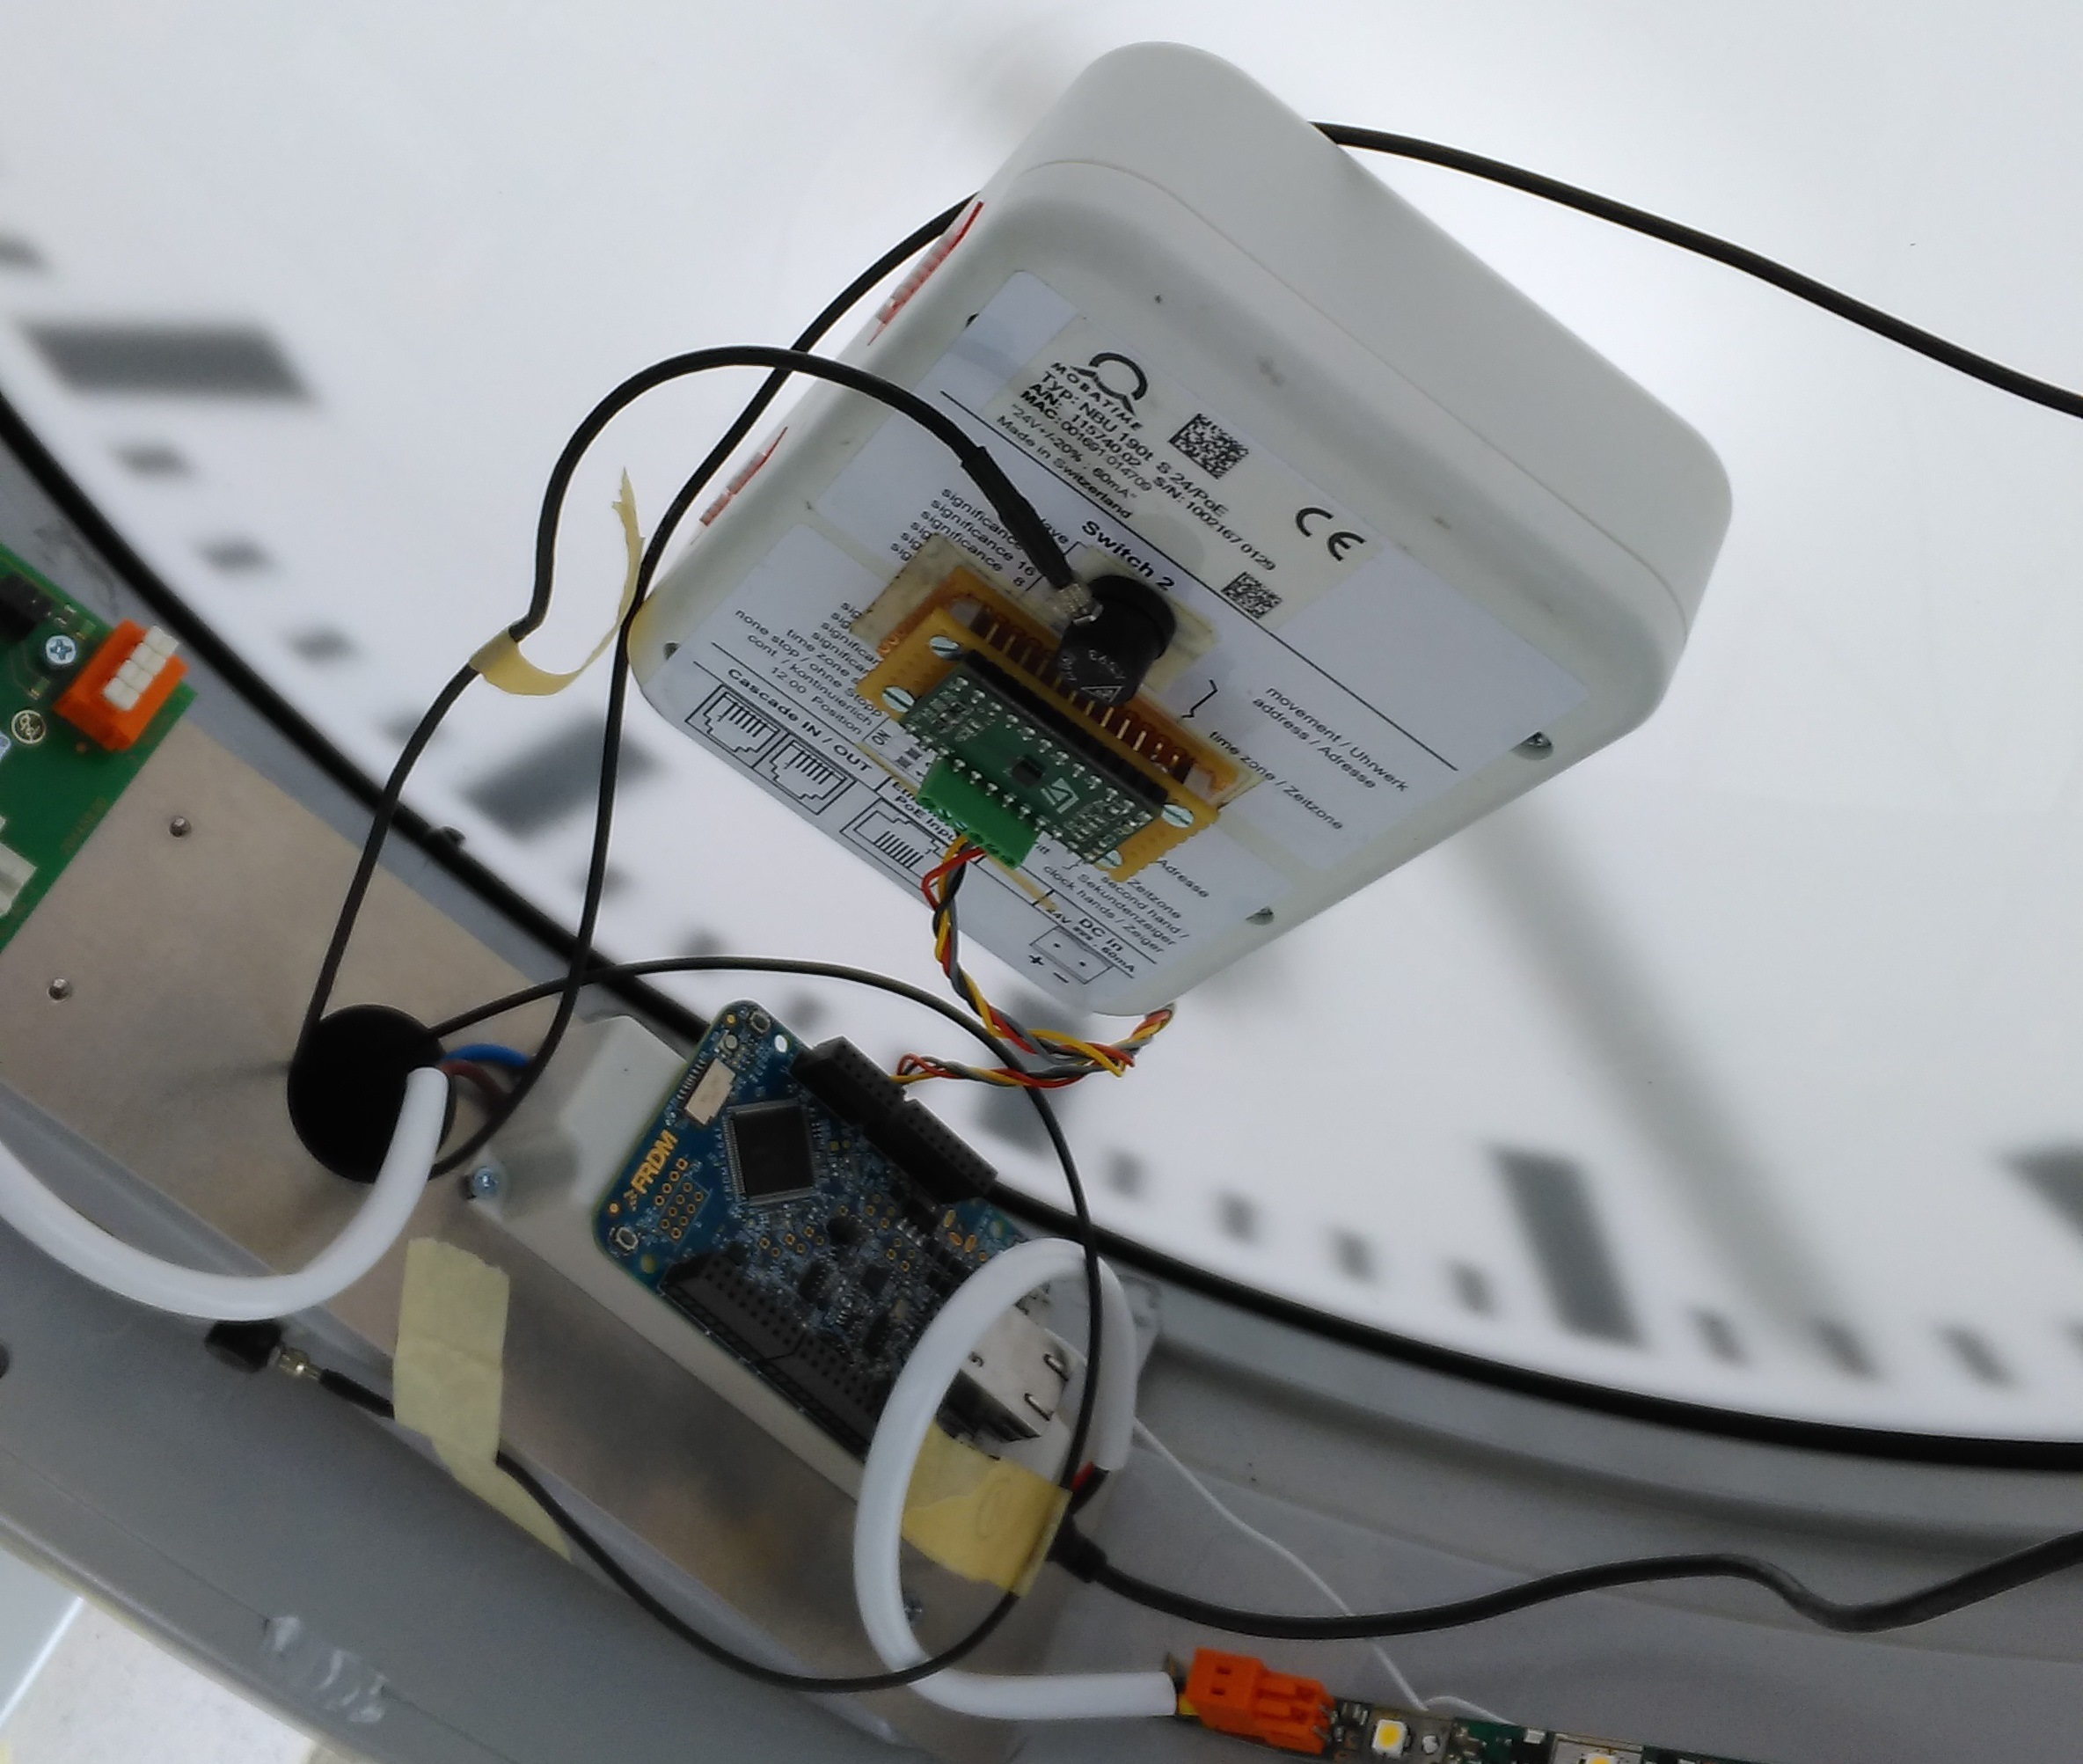
\includegraphics[width=8.5cm]{img/mems_montage2.jpg}
			\caption[Montage Sensoren]{Montage des MEMS Sensors und des pizeoelektrischen Sensors am Uhrwerk}
			\label{fig:mems_montage}
		\end{wrapfigure}
		Die \autoref{fig:vergl_mems_piezo} zeigt die Beschleunigungssignale am Uhrwerk gemessen mit dem
		piezoelektrischen Sensor (blau) wie in \autoref{chap:piezo} und jenen gemessen mit dem MEMS-Sensor
		(rot). Die beiden Messungen unterscheiden sich in der Abtastrate. Der Signalverlauf des
		piezoelektrischen Sensors wird mit dem Oszilloskop mit einer Frequenz von 500kHz abgetastet. Die
		Abtastrate des MEMS Sensor hingegen kann maximal 1kHz betragen. Das Beschleunigungssignal gemessen
		mit dem piezoelektrischen Sensor hat Frequenzanteile, welche durch die tiefere Abtastrate des
		MEMS Sensors nicht mehr vorhanden sind. Diesen Unterschied erkennt man darin, dass die sehr
		kurzen, hohen Beschleunigungspeaks mit dem MEMS Sensor nicht erfasst werden. Mit der Abtastrate
		des MEMS Sensors von 400Hz wird jedoch die f�r diese Anwendung interessante Eigenfrequenz des
		Ziffernblattes von 50Hz erfolgreich sichtbar. Nach dem Nyquist-Shannon-Abtasttheorem muss die
		Abtastfrequenz mindestens doppelt so hoch sein wie die maximale im Signal vorkommende Frequenz. 
		\begin{SCfigure}
			\centering
			%\vspace{-1cm}
			%\captionsetup{width=10cm}
			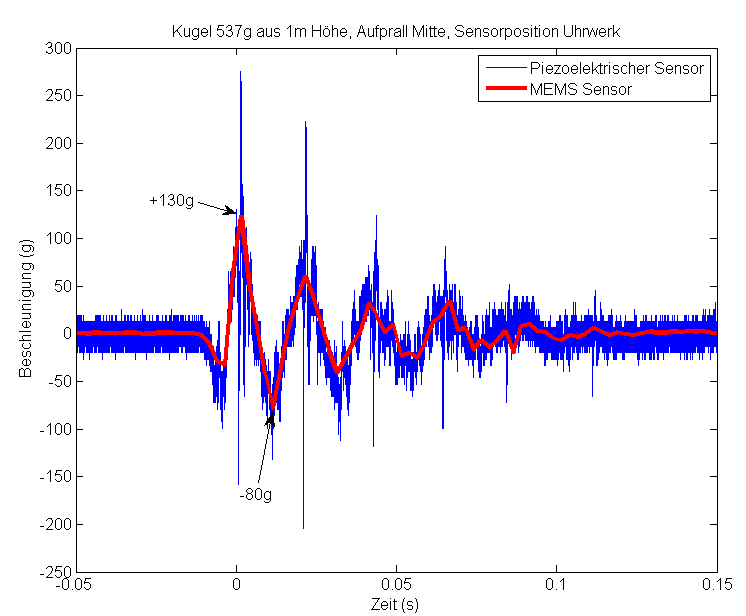
\includegraphics[width=10cm]{img/msg8/vergl_sensoren.png}
			\caption[Vergleich Messung piezoelektrischer und MEMS Sensor]{Beschleunigung bei Aufprall einer Stahlkugel mit einer Masse von 537g aus einer H�he von einem Meter gemessen mit piezoelektrischem Sensor (500kHz, blau)  und dem MEMS-Sensor (400Hz, rot)}
			\label{fig:vergl_mems_piezo}
		\end{SCfigure}
		
		\paragraph{Fazit}
		Mit dem MEMS-Sensor kann mit einer minimalen Abtastfrequenz von 400Hz ein Schock, beispielsweise
		ausgel�st durch einen Steinschlag, detektiert werden. Der Versuch zeigt, dass der mit dem
		MEMS-Sensor aufgezeichnete Beschleunigungsverlauf mit jenem des piezoelektrischen Sensors �berein
		stimmt. Die kurzen und sehr hohen Beschleunigungspeaks werden nicht mehr erfasst. Der Messbereich
		wird dadurch kleiner. Es werden dennoch bei diesem Versuch dennoch Beschleunigungen bis zu 100g
		gemessen. Die f�r die Anwendung interessanten Frequenzanteile von 50Hz sind im Signal enthalten.
		F�r die Anwendung sollte ein Sensor mit einer minimalen Abtastrate von 400Hz und einem Minimalen
		Messbereich von $\pm 200g$ eingesetzt werden. Somit kann der halb so teure Sensor aus der gleichen
		Produktreihe H3LIS200DLTR eingesetzt werden. Dieser hat einen Messbereich bis $\pm 200g$ und 
		eine maximale Abtastfrequenz von 1kHz. Ausserdem ist dieser mit dem f�r den Versuch verwendeten 
		Sensor H3LIS100DLTR pinkompatibel. 
	\newpage	
	\section{Versuch Schock Detektion}
		\paragraph{Vorgehensweise}
		In einem weiteren Schritt wird eine Schock Detektion implementiert und getestet. Der Sensor
		H3LIS331DL hat zwei interne Interrupts. Die beiden Interrupts k�nnen f�r die jeweilige Anwendung 
		konfiguriert werden. Im Kontrollregister wird beispielsweise eingestellt, ob beim �ber- oder 
		Unterschreiten eines bestimmten Schwellwerts der Interrupt ausgel�st werden soll. Optional ist das 
		definieren einer minimalen Zeitdauer, w�hrend derer der Schwellwert �berschritten werden muss. 
		F�r die Schock Detektion Anwendung wird der Interrupt 1 so konfiguriert, dass
		er beim �berschreiten der Beschleunigung auf der z-Achse ausl�st. Der Schwellwert
		und die minimale Dauer des Beschleunigungspeaks werden mittels zweier Registern INT1\_THS und
		INT1\_DURATION gew�hlt. Der Mikrokontroller hat zwei M�glichkeiten, zu erkennen, wann ein
		Interrupt ausgel�st wurde. Einerseits kann der Interrupt Pin des Sensors ausgewertet
		oder das Interrupt Register des Sensors �ber I2C abgefragt werden. Zusammengefasst werden f�r die Schock 
		Detektion folgende Konfigurationen am Sensor vorgenommen: 
		\begin{itemize}
			\item CTRL\_REG3: 0x24. Interrupt Pin high aktiv, push-pull, Interrupts einschalten, Interrupt Signal auf Interrupt Pins verbinden. 
			\item INT1\_CFG: 0x20. Interrupt bei �bersteigen eines Schwellwerts f�r die z-Achse ausl�sen. 
			\item INT1\_THS: gew�nschter Schwellwert f�r die Ausl�sung des Interrupts, 7 bit. 
			\item INT1\_DURATION: gew�nschte Dauer f�r die Ausl�sung des Interrupts, 7 bit. 
		\end{itemize}
		Das Register INT1\_THS wird mit einem 7-bit Wert beschrieben. Der Schwellwert ist abh�ngig vom gew�hlten Messbereich. Er berechnet sich zu 
		\begin{equation}
		Threshold = \frac{Range}{2^7-1} \cdot N = \frac{Range}{127} \cdot N \label{calc:LSBvalue}
		\end{equation}	
		wobei N der im Register INT1\_THS eingetragene Wert ist. 	
		Ein negativer Schwellwert kann nicht definiert werden. �hnlich verh�lt es sich mit dem Register INT1\_DURATION. 
		Es kann ebenfalls mit 7 bit beschrieben werden und kann somit einen maximalen Wert von 127 annehmen. Die Dauer ist abh�ngig von 
		der gew�hlten Abtastfrequenz und berechnet sich zu
		\begin{equation}
		t_{dur} = \frac{N}{ODR}. 
		\end{equation}
		N ist der im Register eingetragene Wert und ODR entspricht der Abtastfrequenz. 
		
		F�r den Versuch wird jeweils das Register INT1\_SRC gepollt und das f�r die z-Achse entsprechende
		Bit abgefragt, welches bei einem Interrupt gesetzt wird. Die Interrupt Bits werden durch 
		einen Lesezugriff auf INT1\_SRC automatisch gel�scht.
		
		\paragraph{Messresultate}
		Um die Schock Detektion zu testen, wurde der Schwellwert durch das Beschreiben des Registers
		INT1\_THS mit dem Wert 4 auf ca. 6g und die minimale Dauer durch das Beschreiben des Registers
		INT1\_DURATION mit dem Wert 1 auf 2.5ms eingestellt. Mit einem Buzzer wird bei einem Schock Event
		akustisch alarmiert und der Schock Event auf die SD-Karte geloggt. In der Software des Mikrokontrollers
		kann eine weitere Bedingung konfiguriert werden. Nach erfolgreicher Detektion eines Schock Events kann f�r 500ms kein
		weiterer Schock mehr geloggt werden. Damit soll verhindert werden, dass ein Schock f�lschlicherweise als mehrere 
		Schocks geloggt wird. Zusammenfassend kann der Schock mit drei Parametern definiert werden: die H�he des Schocks, die Dauer
		des Schocks und die minimal vergangene Zeit seit dem letzten Schock. Die \autoref{fig:test_shockdetect} zeigt einen durch Auf- und Abbewegen des Sensors 
		erzeugten Beschleunigungsverlauf.
		\begin{figure}
			\centering
			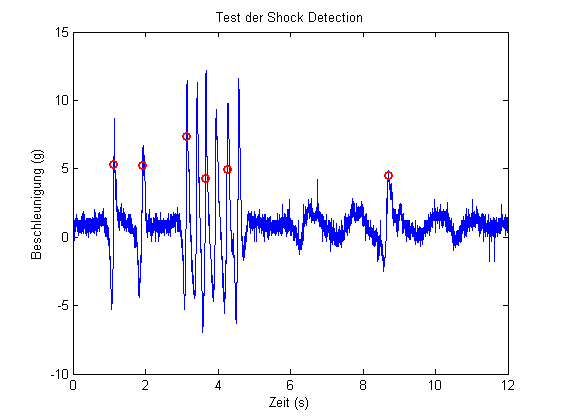
\includegraphics[width=10.5cm]{img/msg9/test.png}
			\caption{Test der Schock Detektion}
			\label{fig:test_shockdetect}
		\end{figure}
		
		 Die roten Punkte markieren die Zeitpunkte, an denen ein Schock detektiert 
		wurde. Die nicht detektierten Beschleunigungspeaks folgen zu schnell auf einen letzten Peak, oder sind zu 
		gering. Es f�llt auf, dass zum Zeitpunkt der Ausl�sung die Beschleunigungswerte jeweils unter 6g liegen.
		Dies liegt daran, dass der Sensor einen Offset aufweist, welcher durch die Software auf dem Mikrokontroller 
		korrigiert wird. Dieser Offset betr�gt ungef�hr 1.7g. Da der Schwellwert jedoch im Sensor intern ausgewertet
		wird, wird entgegen der obigen Berechnung \ref{calc:LSBvalue} der Interrupt um ungef�hr 1.7g zu fr�h ausgel�st. Da bei 
		der Anwendung in der Uhr in einem viel gr�sseren Messbereich gearbeitet wird, spielt dieser Fehler keine Rolle. 
		
		F�r den Test an der Aussenuhr wurden die Parameter Schwellwert und Dauer belassen, nur die minimal vergangene 
		Zeit seit dem letzten Schock wurde auf 200ms reduziert. F�r den Test wurde zweimal die schwere, zweimal die 
		leichte Stahlkugel auf die Aussenuhr fallen gelassen. Nach dreimaligem Aufprall des Softballs und R�tteln 
		an der Uhr, wurde mit der Faust auf die Scheibe geschlagen. Wie in \autoref{fig:shockdetect_uhr} zu sehen 
		ist, verhielt sich der Schock Detektor wie erwartet. Die Kugeln und Faustschl�ge wurden detektiert. 
		Der Aufprall des Softballs (Ann�herung an die Sog-Druckwelle des Zuges) und das R�tteln wurden wie gew�nscht
		nicht detektiert. Dieser Versuch wurde mit der Kamera gefilmt. Bei detektiertem Schock ert�nt ein akustisches
		Signal. Das Video befindet sich auf der CD. 
		\begin{figure}
			\centering
			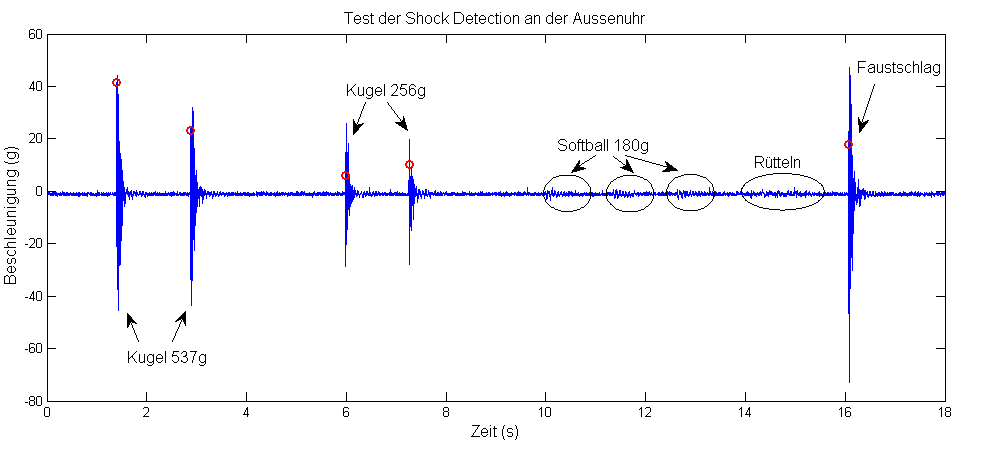
\includegraphics[width=15.5cm]{img/msg10/test_uhr.png}
			\caption{Test der Schock Detektion an der Aussenuhr}
			\label{fig:shockdetect_uhr}
		\end{figure}
		\vspace{-1.5cm}
		\paragraph{Fazit}
		Es wurde ein einfacher Algorithmus implementiert, um ein Schock Event zu detektieren. Dabei wurde die 
		Schock Detektion des Sensors benutzt. Der Sensor bietet die M�glichkeit, einen Schwellwert und eine
		minimale Dauer zu konfigurieren. Erkennt der Sensor einen Schock, so wird ein Interrupt gesetzt. Der
		Mikrokontroller erkennt den Schock indem er das Interrupt Register ausliest oder den Interrupt Pin des
		Sensors abfragt. Zus�tzlich wurde ein dritter Parameter in der Software auf dem Mikrokontroller 
		hinzugef�gt. Dies ist die minimale Dauer seit dem letzten Schock Event. 
		
		Mit diesem einfachen Algorithmus ist es gelungen, Schl�ge zu detektieren. Der Aufprall eines Softballs, welcher 
		eine gr�ssere Kontaktfl�che als zur Folge hat, oder das R�tteln am Rahmen, l�st keine Schockerkennung aus. 
		Es werden nur Einwirkungen auf die Scheibe detektiert. Die Scheibe ist jene Komponente an der Aussenuhr, 
		welche am ehesten besch�digt wird. 
	
	
\chapter{Fazit der Machbarkeitsstudie}



\part{Umsetzung}


\part{Schlussteil}
\chapter{Zusammenfassung}
	Im Rahmen der vorliegenden Arbeit wurde die Machbarkeit einer Schock Detektor mittels Beschleunigungssensoren 
	f�r vernetzte Aussenuhren gekl�rt. 
	
	Die Schock Detektor f�r vernetzte Aussenuhren ist mittels Beschleunigungsmessung grunds�tzlich
	m�glich. Die Versuche mit piezoelektrischen Beschleunigungssensoren haben gezeigt, dass durch
	optimale Platzierung des Sensors am oder im Uhrwerk eine Unterscheidung zwischen Schock Event und
	Druck-Sogwelle eines Zuges realisierbar ist. Schl�ge auf die Scheibe haben grosse
	Beschleunigungen im dreistelligen Bereich am Uhrwerk zur
	Folge. Im Gegensatz dazu misst der an dieser Position befestigte Sensor bei Kr�ften, welche auf
	einer gr�sseren Fl�che wirken, nur kleine Beschleunigungen. Dies ist beispielsweise bei der Druck-Sogwelle eines Zuges
	der Fall. 
	
	In einem weiteren Schritt wurde ein Datenlogger mit dem MEMS Sensor H3LIS331DL entwickelt. Der 
	funktionierende Datenlogger hat gezeigt, dass die Realisierung eines Schock Detektors 
	g�nstig und einfach m�glich ist. Ein Algorithmus mit drei Parametern Schwellwert, 
	minimale Dauer und minimale vergangene Zeit seit dem letzten Schock wurde implementiert und
	erfolgreich an der Versuchsuhr getestet. 
	
	Zum Schluss wurden die verschiedenen M�glichkeiten, einen Schock Detektor im bestehenden 
	Clock Set zu integrieren, zusammengetragen. Die Vor- und Nachteile der L�sungen wurden diskutiert. 
	Die beste Realisierungsidee wurde umgesetzt. Das Schock Detektor Modul kann an die R�ckseite des Uhrwerks montiert werden
	und dient als Datenlogger mit Schnittstelle an einen Computer, kann aber auch an den Clock Controller angeschlossen 
	werden. Messungen an Bahnh�fen und �ber l�ngere Zeit sind unumg�nglich. Die Uhren haben 
	verschiedene Durchmesser und sind verschieden montiert. Mit dem Schock Detektor Modul 
	kann eine umfassendere Messreihe an verschiedenen Bahnh�fen und Aussenuhren durchgef�hrt werden. 
	
	Die folgende Anforderungsliste zeigt die zu Beginn der Arbeit definierten Anforderungen und deren Erf�llungsgrad 
	am Schluss der Arbeit. Die Anforderungen an das Produkt sind zwar Forderungen, mussten jedoch noch nicht
	zwingend im Rahmen dieser Arbeit erf�llt werden. So ist es nicht schlimm, so dass die Zeit nicht gereicht hat, 
	die Software so zu erweitern, dass der Alarm �ber SNMP abgesetzt werden kann. Abkl�rungen 
	zur Realisierung auf den bestehenden ATMEL- Kontrollern wurden insofern gemacht, dass die ungef�hre
	Auslastung der Betriebssysteme bekannt sind. Genauere Untersuchungen folgen, sobald die 
	Software auf dem Schock Detektor Modul in Betrieb ist. Zusammenfassend l�sst sich sagen, dass die 
	zu Beginn der Arbeit definierten Ziele erreicht wurden. Dar�ber hinaus wurde ein erster Prototyp 
	der Schock Detektor als "'Schock Detektor Modul"' realisiert. 
	\newpage
	
	\paragraph{Anforderungsliste}	\label{chap:anforderungen}
	\begin{longtable}{p{0.5cm} p{0.5cm} p{8.5cm} p{0.75cm} p{1.5cm}} \toprule
		\textbf{Nr.}	&  &\textbf{Anforderung} & \textbf{Prio} & \textbf{Erf�l-lungsgrad}\\	
		\midrule
		\endhead
		\multicolumn{3}{l}{\emph{Fortsetzung auf n�chster Seite}}	\\ \bottomrule \endfoot \endlastfoot
		\\
		&		&\multicolumn{2}{l}{\textbf{Anforderungen an die Machbarkeitsstudie}}							
		\\
		1 & 	&	Es ist zu �berpr�fen, ob mit einem Beschleunigungssensor 
		Vandalismus an einer Uhr (Besch�digung Scheibe, Uhrwerk) 
		erkannt werden kann												& F & \cellcolor{green}erf�llt \\ 
		2 &  	& 	Der Vandalismus muss von Windb�en und der Sog-Druckwelle 
		eines Zuges unterschieden werden k�nnen. 						& F & \cellcolor{green}erf�llt \\		
		3 & 	& 	Es sollen verschiedene Schock-Situationen getestet werden.		& F & \cellcolor{green}erf�llt \\
		& 3.1	&	Es soll ein geeigneter Messaufbau entwickelt werden, um 
		die Schock-Situationen zu simulieren. 							&F & \cellcolor{green}erf�llt \\
		& 3.2 & 	Der Messaufbau muss so gew�hlt werden, dass die Messungen 
		reproduzierbar sind. 											&F & \cellcolor{green}erf�llt \\
		4 & 	&	Falls die Detektion m�glich ist, soll ein geeigneter 
		Algorithmus entwickelt werden (z.B. in MATLAB). 				& F & \cellcolor{green}erf�llt \\
		5 & 	& 	Es soll abgekl�rt werden, ob die Implementierung auf dem
		vorhandenem ATMEL- Kontroller realisiert werden kann.			& F & \cellcolor{orange}teilweise erf�llt \\
		&	5.1	&	Falls die Implementierung auf dem ATMEL- Kontroller nicht
		realisiert werden kann, muss abgekl�rt werden, welche
		anderen Komponenten ben�tigt werden.							& F &\cellcolor{green}erf�llt \\
		6 &		& 	Der Stromverbrauch der Produkterweiterung soll abgekl�rt und
		dokumentiert werden.											& F &\cellcolor{green} erf�llt \\
		7 & 	& 	Es soll abgekl�rt werden, ob eine vorhandene Schnittstelle 
		(SPI, I2C, UART) verwendet werden kann.							& W &\cellcolor{green}erf�llt \\
		\\
		&		&\multicolumn{2}{l}{\textbf{Anforderungen an das Produkt}}								
		\\
		1 &		& 	Die Sensorik darf von aussen nicht sichtbar sein.	& F &\cellcolor{green}erf�llt \\
		2 & 	& 	Der Alarm soll mittels SNMP �ber die bestehende Uhrsteuerung
		abgesetzt werden k�nnen.										& F &\cellcolor{red}nicht erf�llt \\
		3 &		&	Die Kosten f�r den Sensor liegen im Bereich von 5 bis maximal 10 Fr.
		pro St�ck.														& F & \cellcolor{green}erf�llt \\
		4 & 	& 	Das Sensormodul soll einfach in der Uhr montiert werden k�nnen.
		Die Platzverh�ltnisse sind insofern beschr�nkt, dass die
		Beleuchtung der Uhr nicht gest�rt wird (siehe Anforderung
		Produkt Nr. 1)													& F & \cellcolor{green}erf�llt \\
		5 & 	&	Das Produkt muss bei einer Betriebstemperatur von -30 bis +70�C 
		arbeiten.  														& F & \cellcolor{green}erf�llt \\
		\bottomrule					 	
		\caption{Anforderungen an die Machbarkeitsstudie und an das Produkt} 
		\label{tab:Anforderungen}
	\end{longtable}
	
	\paragraph{Lessons Learned}
	%\chapter{Lessons Learned}
		Eine Herausforderung dieser Arbeit war, dass Messungen auf dem Perron nicht m�glich waren.
		Deshalb musst eine andere L�sung gefunden werden, abzusch�tzen, was f�r einen Einfluss
		Durck-Sogwellen eines Zuges auf die Beschleunigung in der Aussenuhr hat. Dies hat gezeigt,
		dass nicht nur der auf den ersten Blick offensichtliche Weg zum Ziel f�hrt, sondern mit Geduld ein
		anderer Ansatz gefunden werden kann.
		
		Bei Inbetriebnahme des MEMS Beschleunigungssensors lag die Schwierigkeit darin, dass das
		Datenblatt des �fteren Fragen unbeantwortet liess. So war es zu Beginn nicht klar, wie genau die
		Beschleunigungsdaten interpretiert werden m�ssen.
		
		Bei der Softwareentwicklung des Datenloggers wurde das Gelernte �ber das Betriebssystem
		FreeRTOS das erste Mal richtig angewendet. Die effizientere Inter-Task-Kommunikation mittels Task
		Notifications war jedoch ein neuer Ansatz. Es ist nie ausgelernt!




\begin{appendix}
\part{Anhang}
%%-------------------------------------------------------------------------------
% $HeadURL: http://hb9etc.ch/svn/pluess/tex/da_doku/anhang_ztrafo.tex $
% $Revision: 861 $
% $Author: tobias $
% $Date: 2013-12-23 21:15:48 +0100 (Mon, 23 Dec 2013) $
%-------------------------------------------------------------------------------


\chapter{z-Transformation} \index{z-Transformation|(}
Auf den folgenden Seiten soll kurz und knapp die Theorie �ber die
z-Transformation aufgefrischt werden. Um das ganze m�glichst kompakt zu halten,
werden s�mtliche Beispiele und weitere Erl�uterungen zu den gemachten S�tzen
weggelassen, es wird aber dennoch versucht, die z-Transformation so vollst�ndig
wie m�glich zu erkl�ren. F�r weitergehende Informationen hierzu sei auf
\cite{Frey2008, Lunze2, Froriep} verwiesen.

Die z-Transformation entspricht der Laplace-Transformation, ist jedoch f�r
diskrete Signale vorgesehen.
Die bilaterale z-Transformation ist mit
\begin{equation}
  X(z) = \sum \limits_{k=-\infty}^{\infty} x[k] \, z^{-k}
\end{equation}
definiert. Meist -- auch in der vorliegenden Arbeit -- wird aber die
unilaterale z-Transformation benutzt; diese wird
auch rechtsseitige oder einseitige z-Transformation genannt. Sie ist mit
\begin{equation}
  X(z) = \sum \limits_{k=0}^{\infty} x[k] \, z^{-k}
\end{equation}
definiert. In beiden F�llen ist $z \in \mathbb{C}$.

Die Funktion $X(z)$ heisst Bildfunktion, $x[k]$ heisst
Originalfunktion. Die z-Transformation kann mit $\lap{ x[k] }{ X(z) }$
geschrieben werden; ebenso ist auch $X(z) = \ztransz{x[k]}$ m�glich.


\section{Konvergenzbereich} \index{z-Transformation!Konvergenzbereich}

Die z-Transformierte einer Funktion $x[k]$ existiert nicht zwangsweise f�r
jeden beliebigen Wert von $z$, sondern es gibt auch hier �hnlich wie bei der
Laplace-Transformation bestimmte Bereiche, wo die z-Transformierte existiert
und solche Bereiche, wo sie nicht existiert. Man spricht auch hier wieder vom
sogenannten Konvergenzbereich.

Zun�chst f�hrt man sich die formale Definition der (unilateralen)
z-Transformation
\[
X(z) = \sum \limits_{k=0}^{\infty} x[k] \, z^{-k}
\]
noch einmal vor Augen. Da $z$ eine beliebige Zahl ist, die auch komplex sein
kann, kann sie i.A. als
\begin{equation}
  z = a \, \E^{\j\,b}
\end{equation}
geschrieben werden mit $a,b \in \mathbb{R}$. In diesem Fall ist dann
$a=\abs{z}$ und $b=\arc{z}$. F�r $z^{-k}$ gilt:
\begin{equation}
  z^{-k} = a^{-k} \, \E^{-\j\,b\,k}
\end{equation}
Man erkennt sofort: wenn $a>1$ ist, dann wird f�r wachsende $k$ die
Potenz $a^{-k}$ immer kleiner, und zwar in exponentiellem Masse. Sofern $x[k]$
h�chstens eine exponentiell wachsende Funktion ist, muss die z-Transformierte
also auf jeden Fall existieren, und zwar f�r alle $z$, f�r die $\abs{z}>1$ gilt.
Man erkennt hieraus also: f�r rechtsseitige Funktionen ist der Konvergenzbereich
der z-Transformierten die gesamte komplexe Ebene ausserhalb des Einheitskreises.

F�r Funktionen, die zeitlich begrenzt sind, d.h. nur in einem Intervall
$[k_0, k_1]$ verschieden von 0 sind, und ausserhalb dieses Intervalls
verschwinden (wie z.B. eine Rechteckfunktion), existiert die z-Transformierte
sogar auf der gesamten komplexen Ebene, ausgenommen dem Ursprung. F�r eine
solche Funktion lautet die z-Transformierte n�mlich:
\begin{equation}
  X(z) = \sum \limits_{k=k_0}^{k_1} x[k] \, z^{-k} = x[k_0] \, z^{-k_0} +
  x[k_0 + 1] \, z^{-k_0 - 1} + x[k_0 + 2] \, z^{-k_0 - 2} + \ldots +
  x[k_1] \, z^{-k_1}
\end{equation}
Es gibt also endlich viele Glieder, und daher muss die z-Transformierte auf
jeden Fall konvergieren. Da die Exponenten von $z$ jedoch allesamt negativ sind,
geh�rt der Ursprung der komplexen Ebene aufgrund der Beziehung
\begin{equation}
  z^{-k} = \frac{1}{z^k}
\end{equation}
nicht zum Konvergenzbereich dazu aufgrund der Division durch 0.

Die Funktion $x[k]$ muss allerdings auch noch bestimmten Bedingungen gen�gen,
damit die z-Transformierte existiert. Und zwar darf $x[k]$ h�chstens von
exponentiellem Typ sein. Dies heisst: sei
\begin{equation}
  x[k] < a \, \E^{b\,k}
\end{equation}
und wenn nun f�r jeses $k$ ein $a$ und ein $b$ existiert, f�r die diese
Bedingung wahr ist, dann existiert auch die z-Transformierte. Also:
\begin{equation}
\exists ~ a,b \Leftrightarrow x[k] < a \, \E^{b\,k} ~ \forall k
\end{equation}
Etwas einfacher
kann man diese
Regel auch so formulieren: wenn $x[k]$ nicht schneller als eine
Exponentialfunktion w�chst, dann wird auch eine z-Transformierte existieren.
Funktionen wie $x[k]=k!$ oder $x[k]=\E^{k^2}$ sind daher nicht
z-Transformierbar, da sie schneller als jede Exponentialfunktion wachsen.

\italictitle{Anmerkung}
F�r linksseitige Funktionen $x[k]$ die nur f�r $k<0$ verschieden von 0 sind,
kann eine �hnliche �berlegung angestellt werden wie f�r die rein rechtsseitigen
Funktionen. F�r eine solche linksseitige Funktion gilt n�mlich f�r die
z-Transformierte:
\[
X(z) = \sum \limits_{k=-\infty}^{0} x[k] \, z^{-k}
\]
die Exponenten von $z$ sind somit allesamt positiv. Eine solche unendliche
Reihe kann aber nur dann �berhaupt konvergieren, wenn $\abs{z}<1$ ist. Daher ist
der Konvergenzbereich einer solchen linksseitigen Funktion das innere des
Einheitskreises.


\section{Eigenschaften der z-Transformation}
\index{z-Transformation!Eigenschaften}

\subsection{Linearit�t} \index{z-Transformation!Linearit�t}
Die z-Transformation ist eine lineare Transformation. D.h., es ist:
\begin{equation}
  \ztransz{ a\,x[k] + b\,y[k] } = \ztransz{ a\,x[k] } + \ztransz{ b\,y[k] }
\end{equation}
Zudem gilt auch:
\begin{equation}
  \ztransz{ a\,x[k] } = a \cdot \ztransz{ x[k] }
\end{equation}

\subsection{Verschiebungssatz} \index{z-Transformation!Verschiebungssatz}
Bei einer Verschiebung der Originalfunktion um $k_0$ Zeiteinheiten nach rechts
muss die Bildfunktion entsprechend mit $z^{-k_0}$ multipliziert werden:
\begin{equation}
  \ztransz{ x[k - k_0] } = z^{-k_0} \cdot \ztransz{ x[k] }
\end{equation}
Dies gilt jedoch nur, wenn $x[k] = 0$ f�r $k < 0$ ist. Wenn dies nicht zutrifft,
dann gilt folgendes:
\begin{equation}
  \ztransz{ x[k - k_0] } = z^{-k_0} \cdot \left( X(z) + \sum \limits_{i=1}^{k_0} x[-i] \, z^i \right)
\end{equation}
Der Grund hierf�r ist, dass bei einer Verschiebung nach rechts auf der linken
Seite noch weitere Funktionswerte hinzukommen. Da allerdings i.d.R. nur die
unilaterale z-Transformation benutzt wird und damit $x[k] = 0$ f�r $k < 0$ ist,
ist diese Regel eher von untergeordneter Bedeutung.

Bei einer Verschiebung nach links gilt allerdings immer:
\begin{alignat}{2}
  \ztransz{ x[k] } &= X(z) \\
  \ztransz{ x[k + 1] } &= z \cdot \left( X(z) - x[0] \right) \\
  \ztransz{ x[k + 2] } &= z^2 \cdot \left( X(z) - x[0] - x[1] \, z^{-1} \right) \\
  \ztransz{ x[k + 3] } &= z^3 \cdot \left( X(z) - x[0] - x[1] \, z^{-2} - x[2] \, z^{-3} \right)
\end{alignat}
oder allgemein:
\begin{equation}
  \ztransz{ x[k + k_0] } = z^{k_0} \cdot \left( X(z) - \sum \limits_{i=0}^{k - 1} x[k] \, z^{-i} \right)
\end{equation}

\subsection{D�mpfungssatz} \index{z-Transformation!D�mpfung}
Bei einer D�mpfung eines Signals im Zeitbereich muss folgende Regel beachtet
werden: sei \lap{$X(z)}{x[k]}$, dann gilt
\begin{equation}
  \ztransz{ a^{-k} \, x[k] } = X(a \, z)
\end{equation}
was direkt durch Einsetzen in die Formel f�r die z-Transformation folgt:
\[
  \ztransz{ a^{-k} \, x[k] } =
  \sum \limits_{k=0}^{\infty} x[k] \, a^{-k} \, z^{-k} =
  \sum \limits_{k=0}^{\infty} x[k] \cdot \left(a \, z \right)^{-k}
\]
Dies hat allerdings einen Einfluss auf den Konvergenzbereich. Denn damit die
Summe konvergieren kann, muss $\abs{a\,z} > 1$ sein. Daher ist der
Konvergenzbereich der z-Transformierten: $z>\abs{\frac{1}{a}}$.

\subsection{Lineare Gewichtung} \index{z-Transformation!lineare Gewichtung}
Bei einer linear mit der Zeit gewichteten Funktion gilt folgender Satz:
\begin{equation}
  \ztransz{ k \, x[k] } = -z \cdot \frac{d}{dz} \, X(z)
\end{equation}
Denn die z-Transformierte einer solch gewichteten Funktion lautet
\begin{alignat*}{2}
  \ztransz{ k \, x[k] } &= \sum \limits_{k=0}^{\infty} k\,x[k]\,z^{-k} &&\\
  &= 0 + x[1]\,z^{-1} + 2\,x[2]\,z^{-2} + 3\,x[3]\,z^{-3} + \ldots &&
\end{alignat*}
w�hrend f�r die nicht gewichtete Funktion
\begin{alignat*}{2}
  X(z) &= \sum \limits_{k=0}^{\infty} x[k]\,z^{-k} &&\\
  &= x[0] + x[1]\,z^{-1} + x[2]\,z^{-2} + x[3]\,z^{-3} + \ldots && \quad\vline \frac{d}{dz} \\
  &= 0 - x[1]\,z^{-2} - 2\,x[2]\,z^{-3} - 3\,x[3]\,z^{-4} + \ldots && \quad\vline \cdot (-z) \\
  &= 0 + x[1]\,x^{-1} + 2\,x[2]\,z^{-2} + 3\,x[3]\,z^{-3} + \ldots &&
\end{alignat*}
gilt. Daraus folgt:
\[
 \underbrace{ 0 + x[1]\,z^{-1} + 2\,x[2]\,z^{-2} + 3\,x[3]\,z^{-3} + \ldots }_{ \ztransz{k\,x[k]}} =
 -z \cdot \frac{d}{dz} \, \ztransz{ x[k] }
\]

\subsection{Zeitinversion}\index{z-Transformation!Zeitinversion}
F�r negative $k$ gilt:
\begin{equation}
  \ztransz{ x[-k] } = X\left(\frac{1}{z}\right)
\end{equation}
Denn es ist
\[
  \ztransz{ x[-k] } = \sum \limits_{i=-\infty}^{0} x[k] \, z^{k}
\]
und da
\[
  z^k = \frac{1}{z^{-k}}
\]
ist, folgt hieraus der Zeitinversionssatz.

\subsection{Diskrete Ableitung}\index{z-Transformation!diskrete Ableitung}
Die diskrete Ableitung ist mit
\begin{equation}
  \frac{d}{dz} \, x[k] = x[k] - x[k-1]
\end{equation}
definiert. F�r die z-Transformierte davon gilt:
\begin{equation}
  \ztransz{ x[k] - x[k-1] } = X(z) \cdot \frac{z-1}{z}
\end{equation}
Dies geht aus der folgenden �berlegung mit Hilfe des Zeitverschiebungssatzes
hervor.
\begin{alignat*}{2}
  \ztransz{ x[k] - x[k - 1]} &= \sum \limits_{k=0}^{\infty} \left( x[k] - x[k-1] \right) \, z^{-k} &&\\
  &= \sum \limits_{k=0}^{\infty} x[k]\, z^{-k} - \sum \limits_{k=0}^{\infty} x[k-1]\, z^{-k} &&\\
  &= X(z) \cdot X(z) \, z^{-1} &&\\
  &= X(z) \cdot \left( 1 - z^{-1} \right) &&\\
  &= X(z) \cdot \left( 1 - \frac{1}{z} \right) &&\\
  &= X(z) \cdot \frac{z-1}{z} &&
\end{alignat*}

\subsection{Diskrete Integration}\index{z-Transformation!diskrete Integration}
Das diskrete Integral $I[k]$ einer Funktion $x[k]$ ist wie folgt definiert:
\begin{equation}
  I[k] = \sum \limits_{i=0}^k x[i]
\end{equation}
Die z-Transformierte davon lautet wie folgt:
\begin{equation}
  \ztransz{ \sum \limits_{i=0}^k x[i] } = X(z) \cdot \frac{z}{z-1}
\end{equation}
Dies kann damit begr�ndet werden, dass die Integration als die Faltung
\begin{equation}
  I = x[k] \ast 1
\end{equation}
dargestellt werden kann\footnote{Man beachte: das neutrale Element der Faltung
ist nicht 1, sondern $\delta[k]$.}. Unter Anwendung des Faltungssatzes erh�lt man so:
\begin{equation}
  \ztransz{ x[k] \ast 1 } = \underbrace{X(z) \vphantom{\frac{z}{z}} }_{\ztransz{x[k]}}
  \cdot \underbrace{ \frac{z}{z-1} }_{\ztransz{1}}
\end{equation}


\subsection{Faltungssatz} \index{z-Transformation!Faltung}
Bei einer diskreten Faltung zweier Signale im Zeitbereich werden die
Bildfunktionen miteinander Multipliziert:
\begin{equation}
  \ztransz{ x[k] * y[k] } = \ztransz{ x[k] } \cdot \ztransz{ y[k] }
\end{equation}


\subsection{Anfangswertsatz} \index{z-Transformation!Anfangswertsatz}
Ist die z-Transformierte $x(z)$ einer Funktion $x[k]$ bekannt, so kann direkt
ohne vorg�ngige R�cktransformation der Anfangswert $x[0]$ mit dem
Anfangswertsatz berechnet werden:
\begin{equation}
  \lim \limits_{k \rightarrow 0} x[k] = \lim \limits_{z \rightarrow \infty} X(z)
\end{equation}
Dies folgt unmittelbar durch Einsetzen in die Formel f�r die z-Transformation:
\[
  \lim \limits_{z\rightarrow\infty} X(z) =
  \lim \limits_{z\rightarrow\infty} \sum \limits_{k=0}^{\infty} x[k] \, z^{-k} =
  x[0]
\]
wenn $z$ gegen unendlich geht, dann nimmt n�mlich die Folge $z^{-k}$ so rasant
ab, dass in der Summe nur noch das 1. Glied $x[0]$ �brig bleibt und alle anderen
Glieder zu 0 werden.

\subsection{Endwertsatz} \index{z-Transformation!Endwertsatz}
Analog zum Anfangswertsatz gibt es auch eine M�glichkeit, den Endwert der
Funktion $x[k]$ ohne vorherige R�cktransformation zu berechnen. Dazu dient die
folgende Beziehung:
\begin{equation}
  \lim \limits_{k \rightarrow \infty} x[k] =
  \lim \limits_{z \rightarrow 1} \left(z - 1\right) \cdot X(z)
\end{equation}
Ist  der Endwert der Sprungantwort gesucht, dann kann dieser wie folgt berechnet
werden:
\begin{equation}
  \lim \limits_{z \rightarrow 1} \cancel{ \left(z - 1\right) } \cdot \frac{z}{\cancel{ z - 1} } \cdot X(z)
  = \lim \limits_{z \rightarrow 1} X(z)
\end{equation}
Dies liegt darin begr�ndet dass die Heaviside-Funktion ja die z-Transformierte
$\frac{z}{z-1}$ hat. Die Sprungantwort erh�lt man somit durch Multiplikation mit
$\frac{z}{z-1}$.


\section{Inverse z-Transformation} \index{z-Transformation!inverse}

\subsection{Geschlossene L�sung}

Die inverse z-Transformation kann theoretisch mit
\begin{equation}
  x[k] = \frac{1}{2\,\pi\,\j} \oint \limits_{(C)} X(z) \, z^{k-1} \, dz
\end{equation}
berechnet werden. Dabei ist die Kurve $C$ eine beliebige geschlossene Kurve in
der komplexen Ebene, die komplett innerhalb des Konvergenzbereichs der
z-Transformierten liegen muss und die den Ursprung sowie alle Pole der 
z-Transformierten $X(z)$ umschliesst.
Dies ist jedoch sehr aufwendig. Man behilft sich daher mit
�hnlichen Verfahren wie bei der Laplace-Transformation, d.h. die Bildfunktion
wird mittels Partialbruchzerlegung in bekannte Bildfunktionen zerlegt, die dann
einfach zur�cktransformiert werden k�nnen.

Dabei ist es oft von Vorteil, nicht direkt die Bildfunktion $X(z)$ zur�ck zu
transformieren, sondern die Funktion $\tilde{X}(z) = \frac{X(z)}{z}$. Man
zerlegt also $\tilde{X}(z)$ in Partialbr�che. Anschliessend werden die
einzelnen Partialbr�che wieder mit $z$ multipliziert und dann erst kann die
R�cktransformation der Partialbr�che erfolgen.

Der Grund f�r diesen Umweg ist die im Vergleich zur Laplace-Transformation
prinzipiell andere Form der z-Transformierten. I.d.R. ist es nicht sehr einfach,
eine z-Transformierte direkt r�ckzutransformieren, mit diesem Umweg wird diese
Angelegenheit aber etwas vereinfacht.


\subsection{Rekursive R�cktransformation} \index{z-Transformation!inverse, rekursive}
Nicht in allen F�llen gelingt eine exakte R�cktransformation einer
z-Transformierten, weil u.U. die Partialbruchzerlegung nicht m�glich oder zu
aufwendig ist, oder aber man ist nur an den numerischen Werte interessiert,
nicht aber an der geschlossenen Form der R�cktransformierten.
In einem solchen Fall kann auf die rekursive R�cktransformation
zur�ckgegriffen werden. Wohl liefert sie die einzelnen diskreten Werte der
R�cktransformierten, aber man erh�lt keinen geschlossenen Term zur Beschreibung
des Resultats.

F�r die rekursive R�cktransformation einer Funktion $X(z)$ muss die
z-Transformierte zun�chst in eine Form wie die folgende gebracht werden:
\begin{equation}
  X(z) = \frac{ \sum \limits_{i=0}^M b_i \, z^i }{ \sum \limits_{i=0}^N a_i \, z^i }
  = \frac{ b_0 + b_1\,z + b_2\,z^2 + b_3\,z^3 + \ldots + b_M\,z^M}{a_0 + a_1\,z + a_2\,z^2 + a_3\,z^3 + \ldots + a_N\,z^N}
  \label{zform}
\end{equation}
Die Exponenten von $z$ m�ssen also allesamt positiv sein. Ist dieser Schritt
vollzogen, dann kann die rekursive R�cktransformation mit folgender Vorschrift
vorgenommen werden:
\begin{equation}
  x[k] = \begin{cases}
  0 & k < 0 \\
  \frac{1}{a_R} \cdot \left( b_{R-k} - \sum \limits_{i=1}^R a_{R-i} \, x[k - i] \right) & k \geq 0
  \end{cases}
\end{equation}
Hierbei ist $R$ die Anzahl der Koeffizienten. Ist der Z�hlergrad $M$ verschieden
vom Nennergrad $N$, dann gilt:
\begin{equation}
  R = \max \left\{ M, N \right\} \label{nwert}
\end{equation}
Mit dieser rekursiven R�cktransformation ist es nun also m�glich, die
numerischen Werte der einzelnen St�tzstellen einer Funktion im Zeitbereich zu
berechnen. Voraussetzung hierf�r ist dann allerdings, dass man die
vorhergehenden St�tzstellen bereits berechnet hat. Werte $x[k]$ f�r $k < 0$
werden einfach zu 0 angenommen, damit ist dies eine unilaterale
R�cktransformation.


\section{G�ngige Korrespondenzen der z-Transformation}
\begin{table}
  \centering
  \begin{tabular}{l l l l l} \toprule
  Zeitbereich                     & Bildbereich                   && Zeitbereich                      & Bildbereich \\ \midrule
  $\displaystyle 1$               & $\displaystyle \frac{z}{z-1}$ && $\displaystyle k$                & $\displaystyle \frac{z}{\left(z-1\right)^2}$ \\[1.1em]
  $\displaystyle a^k$             & $\displaystyle \frac{z}{z-a}$ && $\displaystyle \E^{\alpha\,k}$   & $\displaystyle \frac{z}{z-\E^{\alpha}}$ \\[1.1em]
  $\displaystyle a^{k-1}$         & $\displaystyle \frac{1}{z-a}$ && $\displaystyle \cos \omega\,k$  & $\displaystyle \frac{z^2 - z\cos\omega}{z^2 -2\,z\cos\omega + 1}$ \\[1.1em]
  $\displaystyle \delta[k]$       & $1$                           && $\displaystyle \sin\omega\,k$   & $\displaystyle \frac{z\sin\omega}{z^2 - 2\,z\cos\omega + 1}$ \\ \bottomrule
  \end{tabular}
  \caption{G�ngige Korrespondenzen}
\end{table}

\index{z-Transformation|)}

%-------------------------------------------------------------------------------
% $HeadURL: http://hb9etc.ch/svn/pluess/tex/da_doku/anhang_glossar.tex $
% $Revision: 861 $
% $Author: tobias $
% $Date: 2013-12-23 21:15:48 +0100 (Mon, 23 Dec 2013) $
%-------------------------------------------------------------------------------

\chapter{Glossar} \index{Glossar} \index{Abk�rzungsverzeichnis}
%\markboth{Glossar}{Glossar}
%\addcontentsline{toc}{chapter}{Glossar}
\label{glossar}

\begin{description}[style=multiline,leftmargin=2.5cm]
  \item[\bf Queue] Eine Liste mit Eintr�gen, welche abgearbeitet werden sollen. Eine Queue kann
  einen Aufrufer blockieren, falls sie voll oder leer ist. \index{Queue} \index{Queue|see{Queue}}
  
  \item[\bf Mounten] engl. \emph{mount "'montieren"', "'befestigen"'}. Bezeichnet bei Unix sowie
  einigen anderen Betriebssystemen den Vorgang, ein Dateisystem an einer bestimmten Stelle - dem
  Mountpoint - verf�gbar zu machen, damit der Benutzer auf die Dateien zugreifen kann.
  \index{Mounten}
  
  \item[\bf pr�emptiv] engl. \emph{preemptive "'unterbrechend"'}. Der Task mit der h�chsten
  Priorit�t erh�lt die CPU. Tasks gleicher Priorit�t teilen sich die Rechenzeit. Der Scheduler kann 
  einen Task unterbrechen. \index{pr�emptiv}
  
  \item[\bf I2C] engl. \emph{Inter-Integrated Circuit}. I2C ist ein 1982 von Philips Semiconductors (heute
  NXP Semiconductors) entwickelter serieller Datenbus.
 
\end{description}
                 % anhang d, glossar (?)
\end{appendix}

{
\raggedright
\setlength{\bibsep}{3mm}
\interlinepenalty=10000
\bibliography{bibliografie/bibliografie}
\interlinepenalty=100
}

\newpage
\clearpage

\listoftables                            % tabellenverzeichnis
\addcontentsline{toc}{chapter}{\listtablename}
\clearpage

\listoffigures                           % bilderverzeichnis
\addcontentsline{toc}{chapter}{\listfigurename}
\clearpage

%\lstlistoflistings
%\addcontentsline{toc}{chapter}{Listing-Verzeichnis}
%\clearpage



\linespread{0.99}
\printindex                              % sachverzeichnis

\end{document}

%-------------------------------------------------------------------------------
